\chapter{Пещеры из дела Бейлиса}

Именно о пещерах из дела Бейлиса пойдет речь. Само дело о том, как в одной из этих пещер, 20 марта 1911 года, нашли мертвым и обескровленным (крови осталась треть) мальчика Андрея Ющинского и в ритуальном его убийстве подозревался работник кирпичного завода Зайцева – Мендель Бейлис – выходит за пределы этой книги.

Пещеры, упомянутые в деле Бейлиса, привлекли меня в 2013 году во время съемок серии «Киевской амплитуды» про Логово Змия. Хотелось найти и снять, по возможности, все пещеры Кирилловских высот.

В один из съемочных дней мы с Колей Арестовым отправились искать пещеры из дела Бейлиса, предполагая, что они примерно над Богуславским спуском, а где именно – черт знает. Полезли на гору у северо-западного конца Богуславского спуска, напротив улицы Нахимова, и стали продвигаться наверху вдоль забора, осматривая обрывающийся слева склон. Большие деревья загораживали вид на Оболонь. Часто приходилось держаться за доски забора, чтобы не полететь вниз. Всё это показано в фильме.

Таким макаром мы долезли до места, где путь нам преградил обвал. Надо было проползти под забором, обойти обвал и двигаться дальше. За забором оказался конец Шишкинского переулка\footnote{На 2020-й местность сильно изменилась – конец переулка раскопали, соорудив вниз некую строительную грунтовку.}.

Я вспомнил, что в 2005 году я тут лазал с подругой Светой, мы зашли сюда же, пролезли к склону за забор и начали пробираться вдоль него налево. Сейчас я восстанавливаю по памяти, как через некоторое время мы проникли в дыру в заборе и оказались на краю большой ямы глубиной эдак в четыре этажа, а окружностью сложно сказать. Внизу было болотце с черной жижей. Мы стали спускаться по крутому берегу, придерживаясь за палки. Под ногами ехал перемешанный с прошлогодней листвой суглинок. Хотели перебраться на другой берег, однако переменили решение и вернулись той же дорогой, что и пришли – через забор, вдоль забора, через забор в Шишкинский переулок. Глядя на карту, предположу, что сия яма находилась между северо-восточными концами переулков Нагорного и Шишкинского.

Вернусь в год 2013. Прозрев, что попали на Шишкинский переулок, мы с Колей снова полезли за забор и оттуда вдоль него на юго-восток. Всё ждали – вот-вот появятся пещеры, ну хоть одна! Ожидания не оправдались. Мы упорно лезли, прыгали, перебегали, медленно спускались, увязали в грязи. В каком-то месте я ощутил странное – мгновенную, временную близорукость, которая кончилась, как только я миновал это место либо по прошествии нескольких секунд. Наконец мы сошли к одному из ответвлений Богуславского спуска – у северо-западного угла автобазы, в 280 метрах от остатков мыса Кирилловской стоянки.

Стали подниматься по отходящей в сторону тропинке. Скоро она привела нас в рощицу, где стоял памятный крест\footnote{50°28'29"N 30°29'10"E} с надписью  дореволюционным начертанием «В окрестностях сего 12/25 марта 1911 года претерпел мученическую кончину святой отрок Андрей Ющинский». Стало быть, поставившие крест тоже  пещеру не нашли. Неясно, где именно убили Ющинского. В пещере обнаружили тело, а вот где убили – вопрос.

Мы совсем устали, поэтому обшаривать все склоны вокруг уже не оставалось сил. Решили продолжить подъем и по ходу глядеть, не отыщем ли чего. По расчетам, мы должны были повторить путь писателя Короленко, осмотревшего сие место столетие назад, и выйти к улице Нагорной. Передохнули минут пять в роще. Там росли березы, дубы, клены. С материалами дела Бейлиса мы были знакомы тогда отрывочно, поэтому и поиск велся не точечно по предварительному вычислению, как в случае с Кирилловской стоянкой, а в надежде на авось да большой охват области поисков. И получается, что в самое интересное с точки зрения поисков место мы добрались уже не в том состоянии, когда хотелось изучить каждый сантиметр.

Уже потом, заполучив трехтомник судебных протоколов с картой и словесными описаниями, пришло некоторое понимание, где надо искать, но повторно к некоторым местам пробраться не удалось, а возможно затея с поиском пещер заведомо провальная, ибо велика вероятность, что они уничтожены. Но об этом позже.

Мы же пошли наверх тропкой, полагая, что рано или поздно выберемся к Нагорной. Слева от тропки показался глубокий тенистый овраг, заросший всякими растениями и большими деревьями. Я спустился туда. По дну, в бетонном желобе, стекал ручеек, и вокруг него пухла намоченная светлая глина. Я вгруз по щиколотки. Конечно, здорово бы спуститься и проследить, куда этот ручей приведет, но я не стал. На другом берегу оврага велась стройка кажется особняка. Я поднялся на прежний берег.

Дальше тропа привела на прямоугольную поляну – как я узнал позже, она называется Стрельбище. Налево отходила старенькая лестница, а прямо была подпорная стенка комплекса «Авангард». На пеньках или лавке под деревом сидел подросток. Забыл тут невесть что. Мы с Колей свернули к лестнице, потом дорожкой между мусорными кучами, вдоль нагромождения сараев и забора по правую руку, затем снова направо, прямо, прямо – и таки вырвались на улицу Нагорную.

Чтобы разобраться, где была пещера с телом Андрея Ющинского, а купно с нею группа смежных пещер, надо обратиться не только к делу Бейлиса, но также продолжить изучать историю местности, где была обнаружена Кирилловская стоянка.

Вспомним карту Хвойки «Общий план части Подола и Оболони», которую я приводил в главе о Кирилловской стоянке. Буквой «B» там помечен мыс с «Кожевником», а к нему с северо-запада примыкал другой мыс, срытый Зайцевым, на кирпичном заводе коего работал Бейлис. По месту срытого мыса было глинище, карьер, а теперь там плоско и автобаза. Буквой «D» обозначена усадьба Зарембского – к северо-западу от исчезнувшего мыса Кирилловской стоянки был еще один мыс, б\'ольшего размера. Автобаза или кирпичный завод Зайцева сожрали часть и этого мыса, а часть уцелела – именно по ней мы с Колей поднимались тропинкой к памятному кресту.

На восточном склоне сего мыса, примыкавшего к мысу Кирилловской стоянки, Хвойка обозначил пещеры. Это значит, что они, все или часть, были вероятно срыты вместе с северным склоном мыса усадьбы Зарембского (позже Бернера). Однако надо тщательно исследовать местность на запад от креста – быть может, там от пещер что-то уцелело.

Далее, на юго-восток от усадьбы Зарембского, Хвойка обозначил буквой «C» то, что в украинском варианте карты записано как «могилы». Что было в русском варианте – могилы или курганы – я не знаю. Теперь там постройки – имущественный комплекс ООО «Славянский дом ФПУ», ранее гостинично-спортивный комплекс «Авангард». Хвойка в статье 1901 года «Каменный век среднего Приднепровья» вскользь упоминает «ряд курганов, находящихся в усадьбе гг. Зарембских».

Автобаза, уже знакомая нам по Кирилловской стоянке, возникла на месте карьера кирпичного завода и окрестностей\footnote{Автобазы вообще как нарочно появляются в местах, имеющих историческую ценность. По сообщению археолога Дмитрия Телегина\cite{telegin01}, до 1970-х годов, эдак в километре на юг от озера Синего (что близ Виноградаря), в окрестностях Берковцов по северной части улицы Маршала Гречко (это уже я предполагаю), в поле была группа из более чем десяти курганов! Конечно же, их уничтожили, построив там автобазу.}. В свою очередь, кирпичный завод был построен Зайцевым на территории усадьб Багреева и Зиваля, причем у Багреева наверху уже был свой кирпичный завод – надо полагать, зайцевский поглотил его.

Сахарозаводчик Зайцев Иона, а точнее Йойна, приобрел упомянутые усадьбы в 1899 году. До того, Зайцев уже владел смежной землей, примыкающей к Кирилловской улице, где несколькими годами ранее построил первый корпус еврейской хирургической больницы. Сейчас, как и прежде, этот дом имеет адрес Кирилловская 61. Здание больницы на 25 коек спроектировал архитектор Карл Шиман. Привожу фотографию, ибо это хороший ориентир. Сейчас дом выше на один этаж, но всё равно узнаваем по узору.

\begin{center}
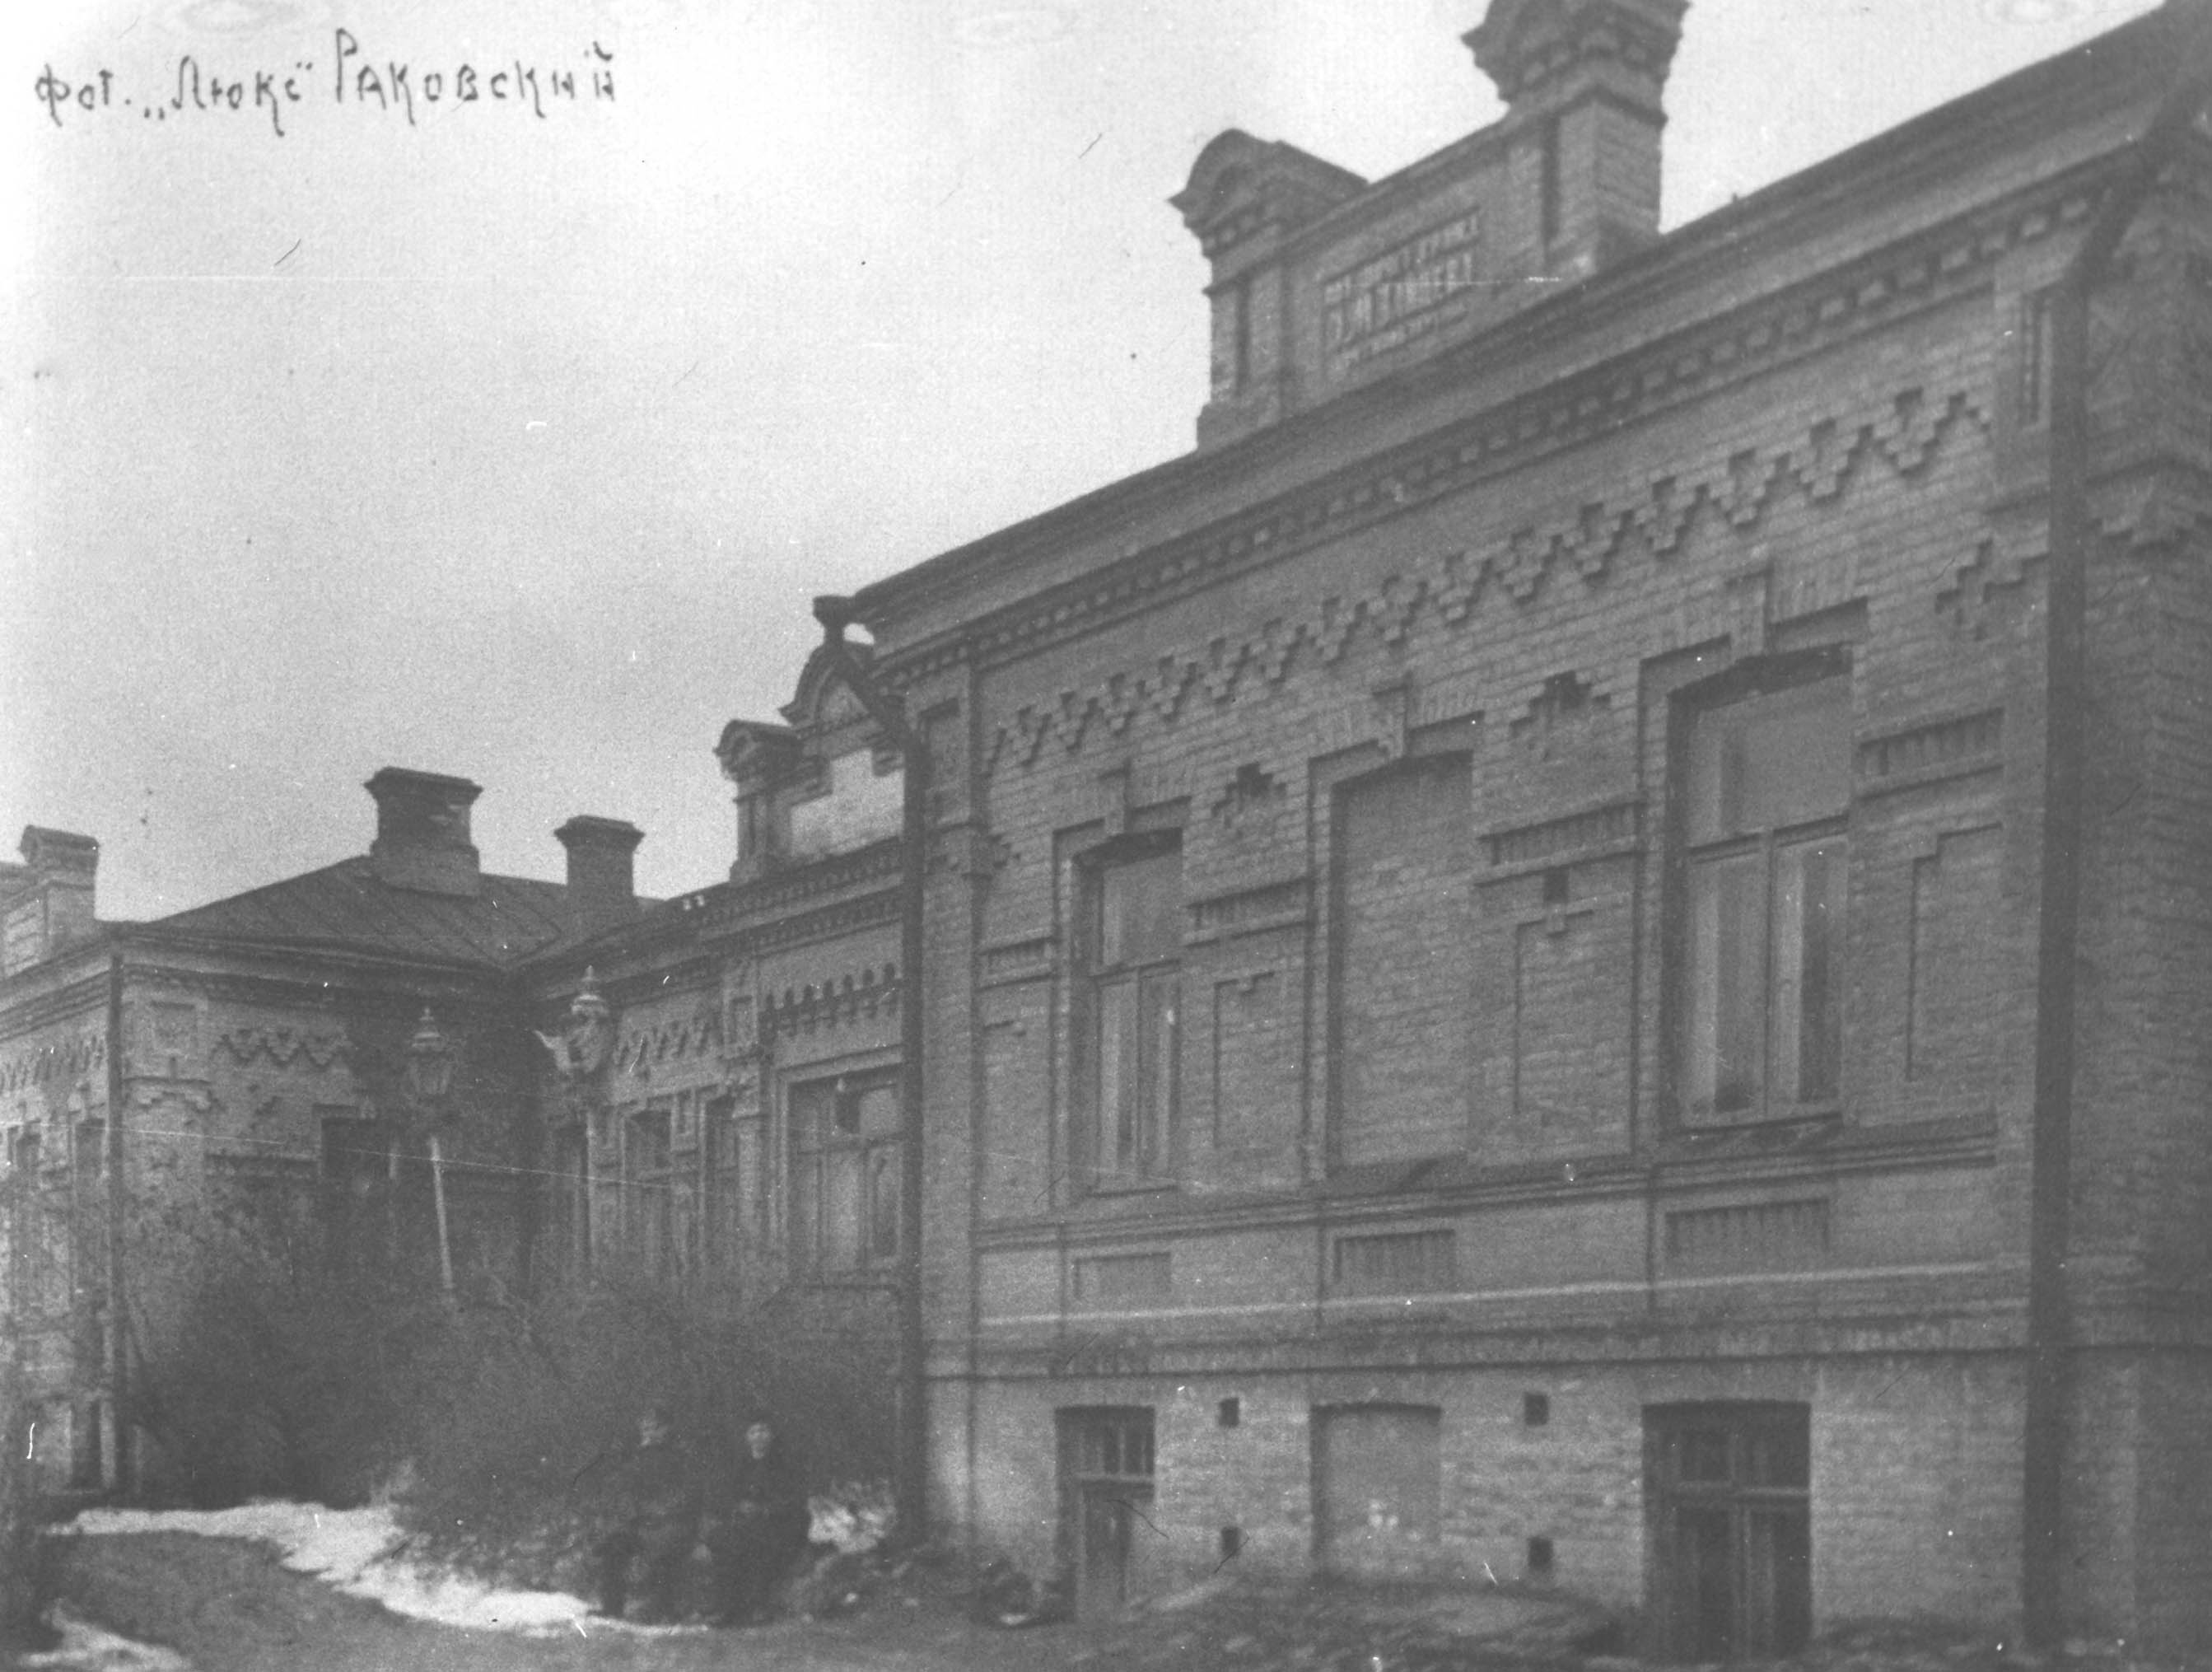
\includegraphics[width=0.90\linewidth]{chast-kirvys/beylis/zaicev-boln-perv-korpus-1920.jpg}

\textit{Еврейская больница Зайцева, фотография 1920-х годов.}
\end{center}

И вот в 1899 году Зайцеву принадлежала уже вся местность на этом отрезке Кирилловских высот, от Кирилловской улицы и наверх. Предприниматель развернул деятельность. Был срезан холм Кирилловской стоянки, на месте его вырыто так называемое глинище – карьер, что заметен на немецкой карте 1918 года залитым водой. Видимо, там образовалось озеро, как по соседству в карьере за кирпичным заводом Рихерта.

%Надо вернуться в прошлое и представить себе, что где было. Сопоставляя фотографии, карты и письменные свидетельства, попытаемся разобраться хотя бы приблизительно, где и до какого времени находились искомые пещеры. 

Дореволюционный снимок, сделанный со стороны Кирилловской стоянки. Фотограф стоит спиной к огрызку ее отрога.

\begin{center}
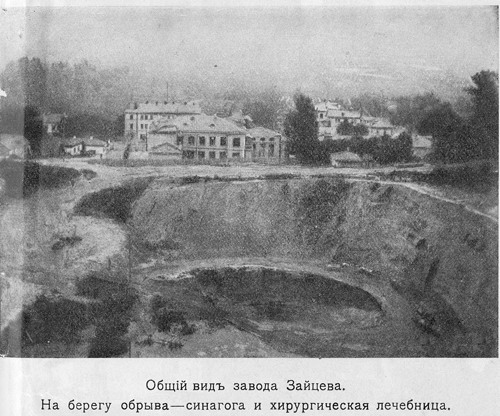
\includegraphics[width=\linewidth]{chast-kirvys/beylis/zavod-zaiceva.png}
\end{center}

Перед нами «глинище» – карьер. За зданием на переднем плане, а это теперь Кирилловская 63 (на некоторых планах 61-А) – Кирилловская улица, и через дорогу за нею, ниже, маячит трехэтажный дом. А вот справа от номера 63 должен стоять старый, первый корпус больницы Зайцева, дом 61 – но я его не вижу. Может потому, что он был одноэтажным с полуподвалом, и скрывается за деревьями. 

В 1907 года Иона Зайцев умер, дела перешли к его сыну Маркусу. В 1911 году под руководством архитектора Эдуарда Брадтмана построили второй корпус (Кирилловская 63), для богадельни со столовой. Под видом столовой делалась синагога (пристройка к зданию, на фото она справа). Вскоре после того, как в печати объявили о закладке новых зданий больницы, по Киеву разнеслась весть о нахождении в близлежащей пещере тела убитого Андрея Ющинского. К 1912 годах строительство новых зданий завершили\footnote{Что до сведений про устроение здесь в 1913 году родильного дома, то предположу, что это наложение данных об открытии Акушерской клиники женского медицинского института в усадьбе Кирилловской земской больницы (там теперь психбольница им. Павлова).}. 

% То бишь открытие сей клиники трактуют как открытие роддома при больнице Зайцева.

%\footnote{Его особняк, построенный по проекту архитектора Владимира Николаева, поныне стоит в Киеве по адресу ул. Грушевского, 20/1, напротив Рады.}
После революции Маркус Зайцев бежал в Одессу и эмигрировал во Францию, Париж, где умер в 1930 году. Больничный комплекс стал непонятно чьим. Его начали растаскивать на части, как это бывает с брошенными зданиями, но в 1922 году  больницу подхватило Общество предоставления помощи бедным больным, на деньги американской еврейской организации Joint. В корпусе богадельни заработала больница на 30 коек (24 – хирургия, 6 – гинекология). Затем здания были национализированы советским правительством.

С 1941 вплоть до 1991 год, там помещался Подольский роддом, или Киевский городской родильный дом №2, которого в год гибели СССР перевели на улицу Мостицкую, 11. «Роддом на Подоле» был местом рождения почти всех подольцев, да и младенцев из других районов. 

В разные времена в бывшей больнице Зайцева работали также институт переливания крови да инфекционная детская больница. В 1958 году по проекту архитектора Солдатова корпуса надстроили на один этаж. С 1991 года они пустовали, а в первом десятилетии 21 века в них расположилась компания «Фармак». 

В археологической литературе часто встречается упоминание «в усадьбах на улице Фрунзе 59, 61» применительно к Кирилловской стоянке, как записано в ее охранном паспорте. Но Кирилловская стоянка отнюдь не на заднем дворе «больничного квартала», а в 180 метрах на северо-запад от Кирилловской 61, за автобазой. Исследовать задворки же между корпусами и Богуславским спуском, невозможно – хода нет, кованные ворота с электронными замками, шлагбаумы.%, пресловутая частная собственность.% Быть может, где-то там сохранились остатки пещер. %Это относится и к зданиям на северо-запад дальше по Фрунзе, следующих за 61-А: 63, 63-А, 65 – хлебкомбината №2 Киевхлеба. Кажется, частично склон доступен со стороны проулка рядом с Фрунзе 69, но я не лазал.

\newpage
\vspace*{\fill}
\begin{center}
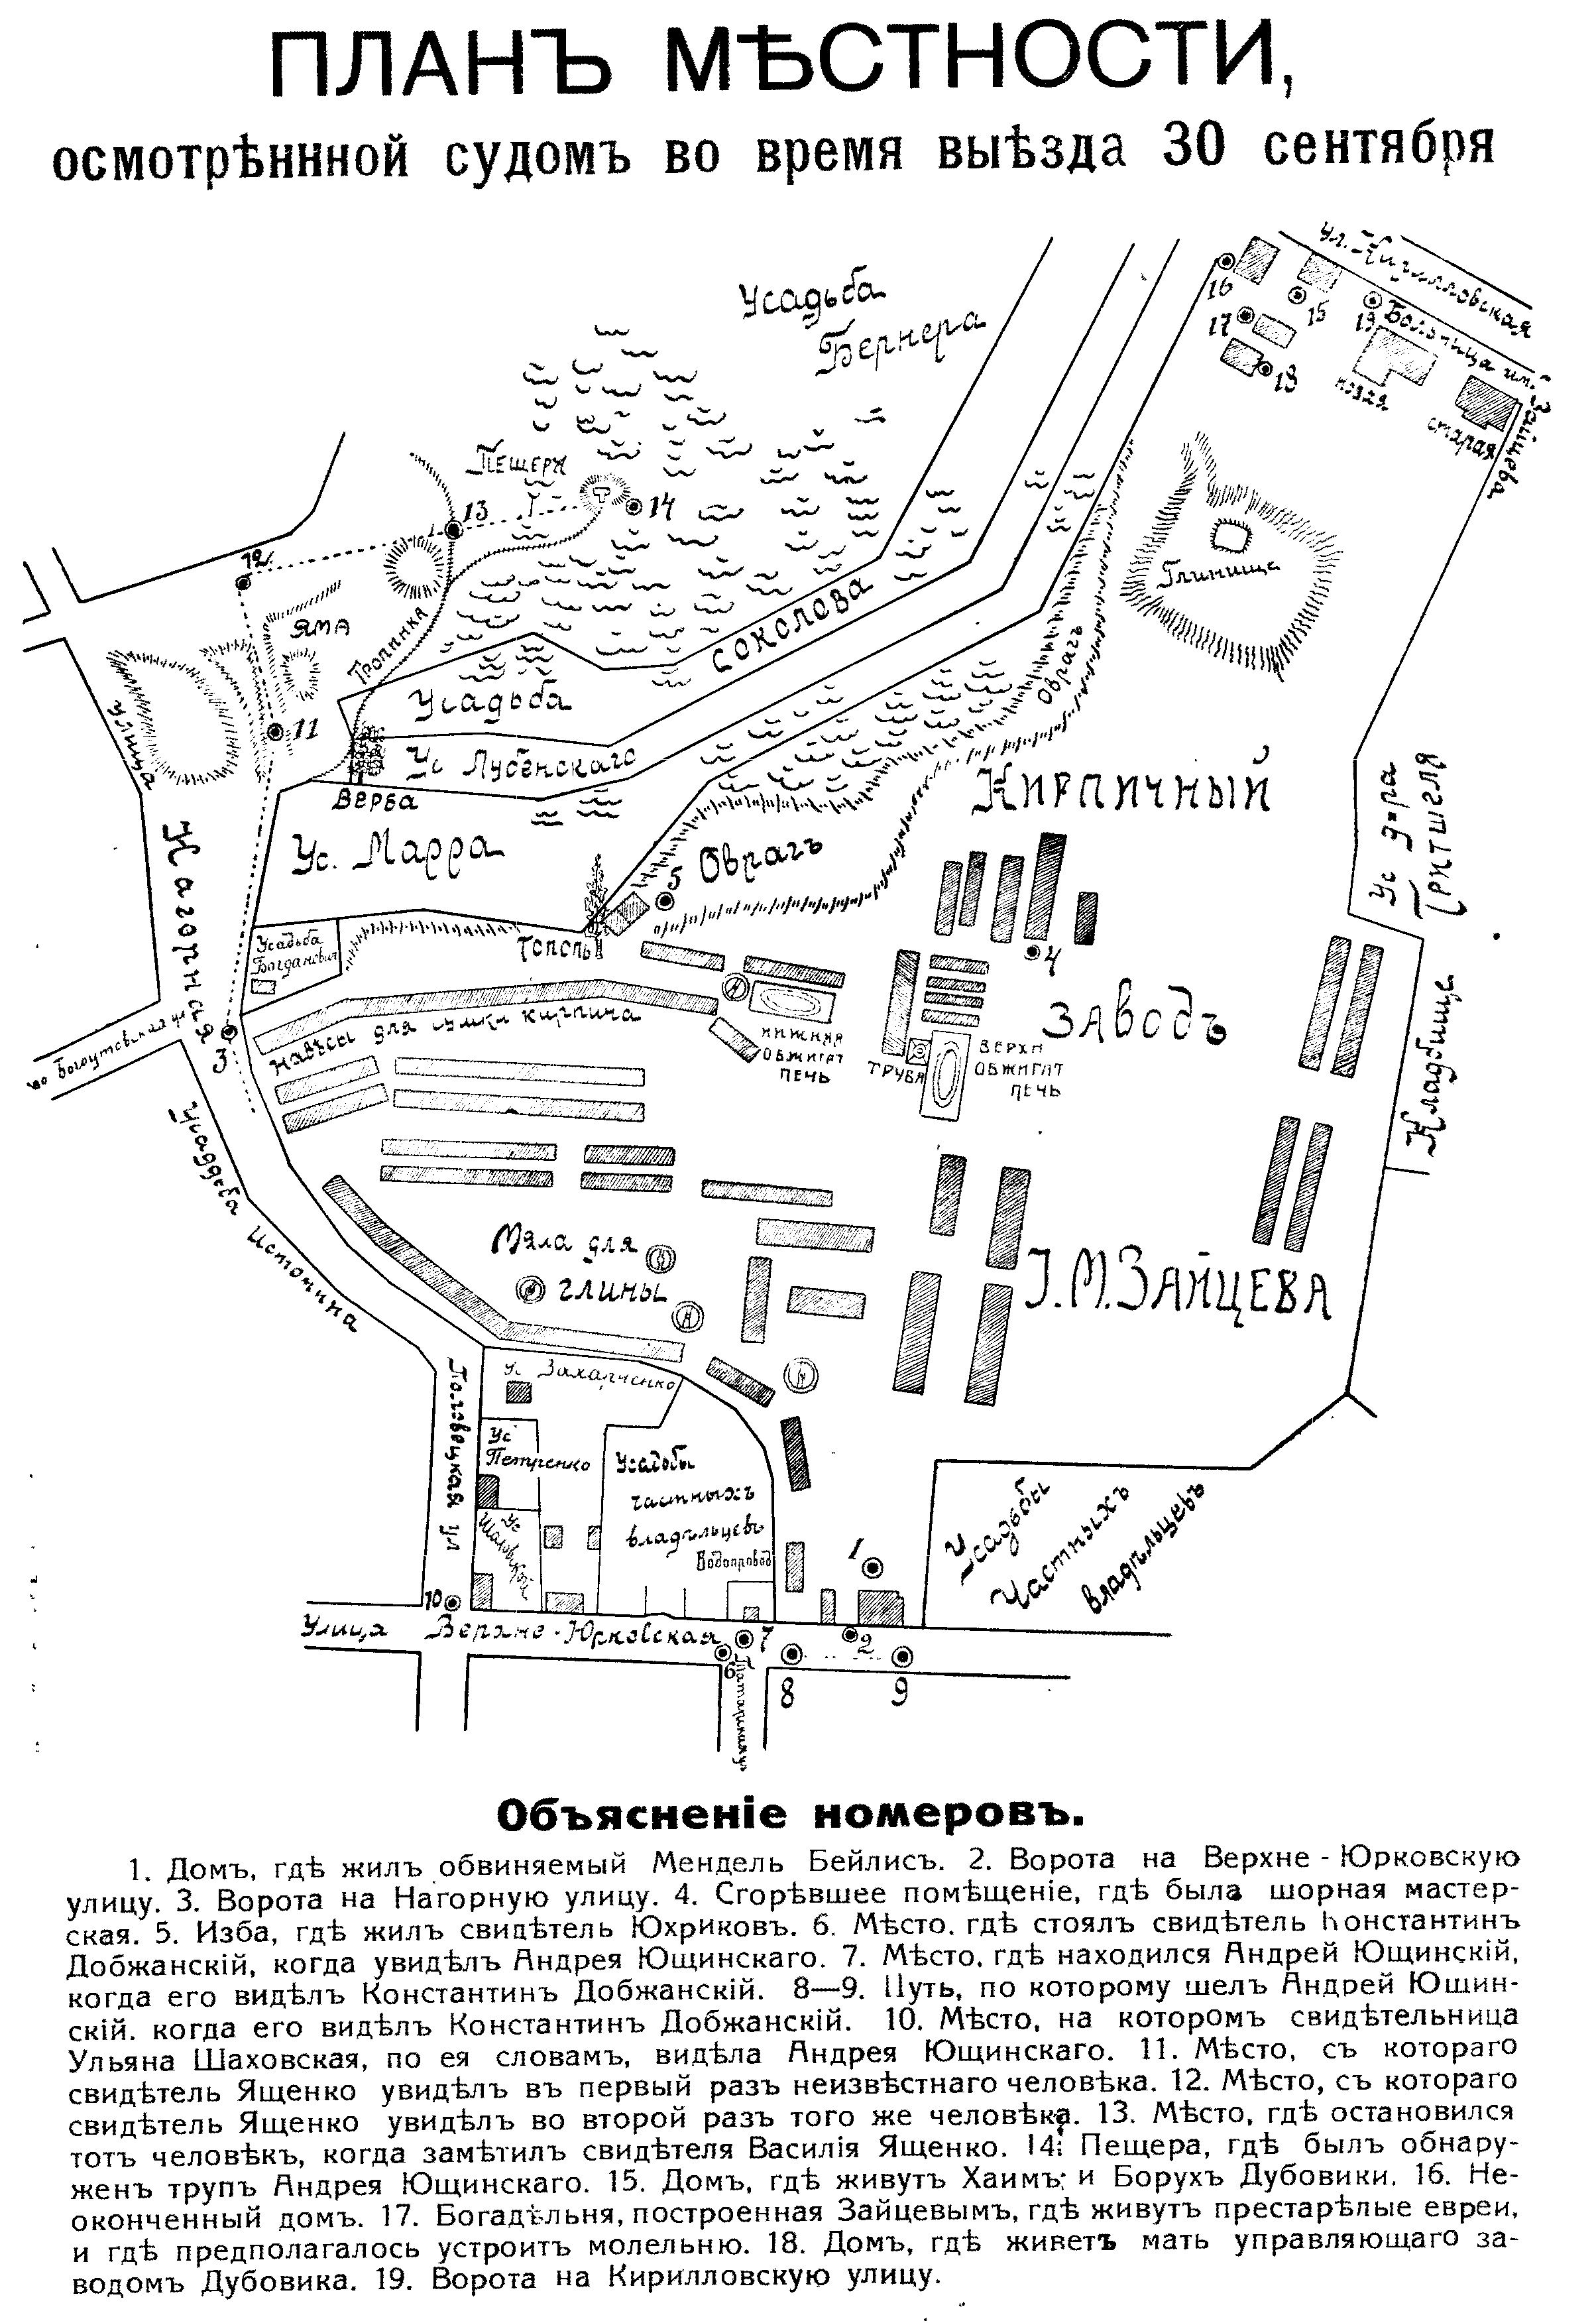
\includegraphics[width=\linewidth]{chast-kirvys/beylis/1913-karta.jpg}
\end{center}
\vspace*{\fill}
\newpage

Карта из трехтомника материалов по суду над Бей\-лисом\cite{beylisdelo} – настоящее сокровище для краеведа! Хотя я не уверен, что под номером 14 на ней обозначено истинное положение пещеры, где нашли тело Андрея Ющинского.

Карта составлена в 1913 году. Она правильно ориентирована на север, однако пропорции объектов, кажется, не везде соблюдены. Это набросок, позволяющий иметь подробное представление о местности с соответствием взаимного расположения объектов. Тогда, в 1913 году, по ней можно было пройти, пользоваться ею, потому что существовали все указанные на карте ориентиры.

Основные постройки завода – над глинищем на холме, практически до самой улицы Верхне-Юрковской. Глинище теперь перекрыто автобазой – но в какой мере? У нижнего правого угла глинища надо полагать, по состоянию на 2017 год, остатки отрога Кирилловской стоянки. Глинище было на месте срытого отрога горы.

В верхнем правом углу – отрезок Кирилловской улицы. На нем под нумером 19 – «больница Зайцева», корпуса помечены как «старая» – это теперь Кирилловская 61, и «новая» – Кирилловская 63. Отмеченный на карте овраг – возможно тот самый, куда я спускался, когда мы с Колей Арестовым шли от креста к Нагорной улице. Кладбище справа – это, конечно, часть Иорданского кладбища на мысе дач «Кожевника».

В сети я нашел еще одну карту – правда, скан ужасного качества. Судя по использованию шестиконечной звезды, это из некой книги сторонника версии ритуального убийства, а таковая большая была одна – «Убийство Андрюши Ющинского: Исследование в 3 ч» Георгия Замысловского, напечатанная в 1917 году. Не могу её достать, поэтому не знаю, верно ли мое предположение об источнике карты. Цифрой 1 в звезде обозначена пещера, цифрой 2 – проем в заводском заборе.

Насколько могу судить, на этой карте видны террасы над глинищем, а к востоку от него – ручей, текущий вдоль мыса дач «Кожевника». Карта выглядит перерисовкой плана 1913 года из трехтомника по делу. Упрощена в пользу выдвигаемой версии, но ценность представляют подробности рельефа, часть которых вызывает у меня вопросы в трактовке. Например, что за кривая линия, берущая начало справа от глинища? Ручей, который протекает вдоль мыса дач «Кожевника»? 

\begin{center}
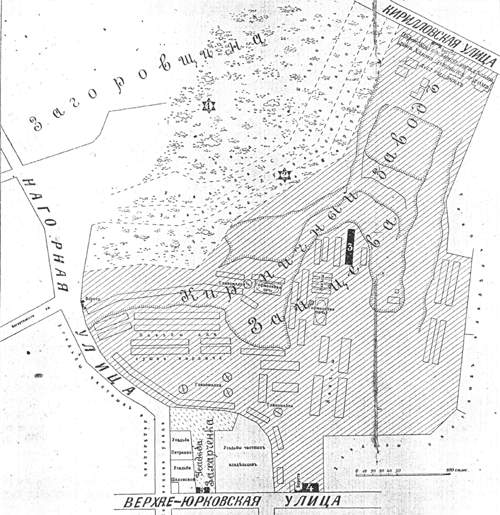
\includegraphics[width=\linewidth]{chast-kirvys/beylis/190x-beylis-karta.jpg}
\end{center}

%Помимо карт, какие есть письменные свидетельства о пещере или пещерах? Их немного. Рассмотрим все.

Писатель Владимир Короленко, современник дела Бейлиса, в 1913 году в статье «На Лукьяновке» рассказал, как побывал на месте действия. Привожу оттуда  выдержки, по которым прослеживается, каким путем писатель шел к пещере.

\begin{quotation}
Вагон трамвая доставил нас к церкви св. Феодора на Дорогожицкой\footnote{Ныне – перекресток Багговутовской и Овручской, близ дома по Овручской, 7.}, откуда мы пошли по узким, своеобразным улицам. Киев вообще стоит в разных плоскостях, но здесь, на окраинах, эта топографическая особенность становится необыкновенно причудлива. [...]

Мы приближаемся к Лукьяновке, к знаменитой отныне усадьбе Зайцева. [...]

Мы на углу Верхней Юрковской\footnote{Верхнеюрковская – часть бывшей улицы Юрковской или Большой Юрковской, что распадалась на Нижнеюрковскую и Верхнеюрковскую. Применительно к году 2017, Верхнеюрковской можно считать улицу Отто Шмидта. С ней под прямыми углами соединяются улицы Печенежская, Татарская и Половецкая.} и Половецкой. Второй от угла двухэтажный деревянный домик\footnote{На фотографиях – кирпичный дом. Стоял примерно напротив нынешнего домика на Отто Шмидта, 33.}. В нижнем этаже над дверью вывеска – «монополия». Здесь, в верхнем этаже, жили супруги Чеберяковы. [...]

Мы идем за угол, по Половецкой...\footnote{От нынешнего перекрестка Отто Шмидта, Багговутовской и Половецкой, Короленко свернул на север и пошел по Половецкой к улице Нагорной, как и следует далее по тексту. От перекрестка уже с Нагорной, на северо-восток, лежали кирпичный завод Зайцева и мыс Кирилловской стоянки.} Направо большая прореха в заборе и невдалеке от забора хибарка. Она имеет вид какой-то опущенности и убогости. Ход из нее на Нагорную – очевидно, для удобства – в эту прореху, заменяющую калитку. Вообще здесь щели, прорехи и лазы разного рода – дело обычное. В хибарке живут супруги Шаховские\footnote{А по карте из протоколов суда, Шаховские жили на углу Верхне-Юрковской и Половецкой.}. [...]

Минуем усадьбу Шаховских и идем дальше. Навстречу беспечной походкой школьников, гуляющих в праздник, идут двое мальчиков-подростков. Один в гимназической шинели. Оба в таком возрасте, что легко могли быть товарищами Ющинского. Мы заговариваем, и юноши охотно останавливаются и дальше поворачивают с нами.

Улица делает угол и ныряет между двух откосов. Направо к откосу, отделяющему улицу от усадьбы Зайцева, лепится очень высокий, но, очевидно, и очень непрочный забор, придающий улице мрачный и характерный вид. Он устроен странно, как бы в два яруса, и в некоторых местах в нем виднеются такие же недавние, как и забор, заплаты. 

   – Хотите посмотреть «мялья»? – спрашивает наш чичероне и указывает на щели в заборе. Мы охотно подходим и заглядываем в эти щели: о «мялах» много говорили в суде.

В щель виден двор кирпичного завода, навесы, клади кирпича. Невдалеке виднеется вертикальный столб, на столбе длинный горизонтальный шест. Тут разводили глину и мяли ее. Для этого к горизонтальному шесту запрягали лошадь, а внизу прикрепляли тяжелые колеса (кажется, от старых лафетов). Лошадь шла по наружному кругу, колеса под шестом бегали внутри и месили глину. [...]

Пока мы смотрим в щели забора, к нам по Половецкой подходят один за другим новые любопытные. [...]

Мы огибаем заборы зайцевской усадьбы, проходим мимо усадьбы Марра\footnote{Это не усадьба Марр с пивзаводом на Кирилловской, но другая усадьба, на улице Нагорной.} и подымаемся на пустырь, поросший лесом. 

Это усадьба Бернера и «Загоровщина», куда так влекло Андрюшу вместо училища... Трудно представить себе место, более привлекательное для детей. Гора широким склоном спускается к Кирилловской улице. Внизу, за ней, точно на плане, лежит чей-то кирпичный завод; видны навесы, высокие трубы и «мяла». За заводом – широкая синяя даль, подернутая легкой дымкой, луга, излучины Почайны и далеко, на самом горизонте, прерывистая лента Днепра. Луговой и днепровский ветер налетает сюда широкими, ласковыми взмахами. [...]

Среди разговоров мы минуем большой глинистый курган, поросший травой... В нем виднеется пещера.

  – Нет, это еще не та...

Та оказывается в нескольких шагах дальше, там, где начинается склон к Кирилловской улице и приднепровским лугам. Холмик разрыт... Видна обнаженная глина. Два дерева выросли на вершине холма, соединенные корнями. Под этими корнями зияет темный ход, довольно круто, коридором уходящий вглубь. В конце этот коридор пересечен узким и коротким ходом накрест, как делают обыкновенно кладоискатели... В одном из концов этого креста и нашли прислоненным в темном углу тело несчастного Андрюши Ющинского... [...]

Назад мы возвращались более кратким путем, наискось с горки, на Нагорную улицу. Влево уходила Половецкая улица с ее высоким забором и глинистым откосом.
\end{quotation}

\vspace*{\fill}
\begin{center}
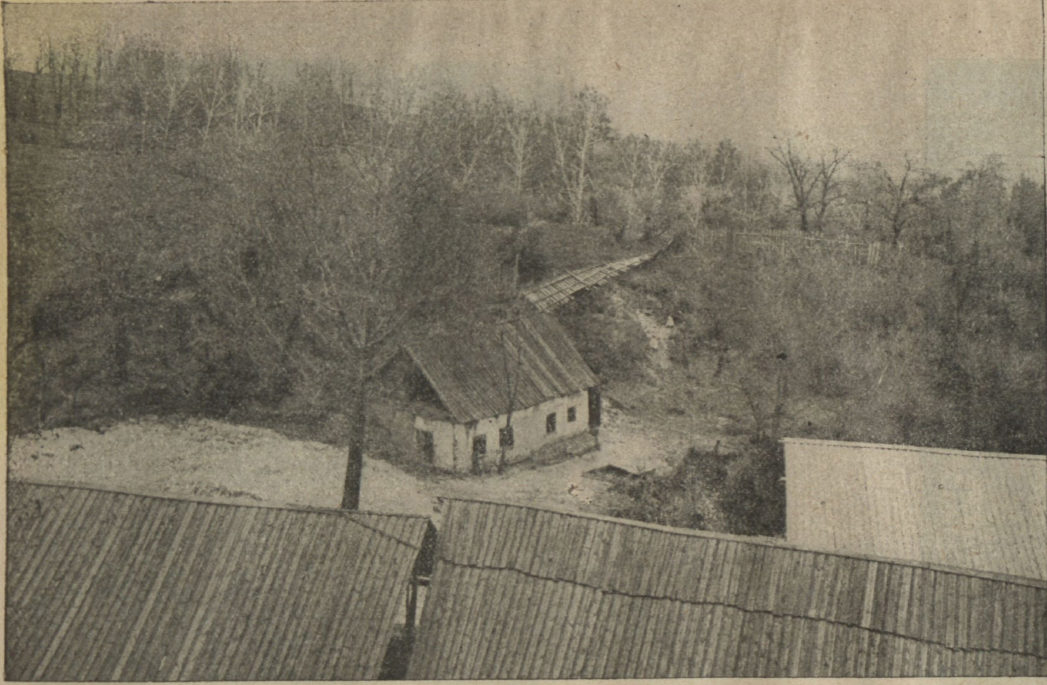
\includegraphics[width=\linewidth]{chast-kirvys/beylis/1912-beylis-storojka.jpg}
\textit{Сторожка на заводе Зайцева.}
\end{center}
\vspace*{\fill}
\newpage

\begin{center}
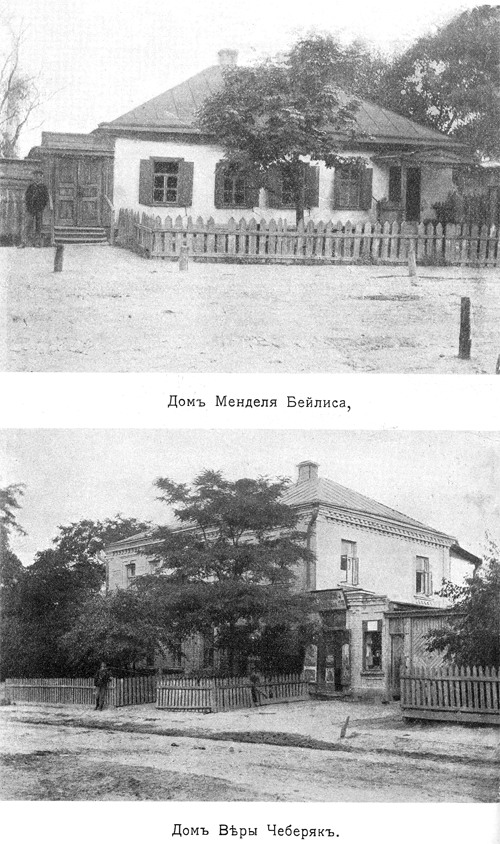
\includegraphics[width=\linewidth]{chast-kirvys/beylis/beylis-houses.jpg}
\end{center}


\newpage


Кирпичный завод, о котором пишет Короленко – это не завод Зайцева. Короленко, зная о заводе Зайцева, наблюдаемое именует «чей-то кирпичный завод» – стало быть, отличает его от завода Зайцева.

В 1913 году усадьба завода Зайцева граничила с улицами Кирилловской, Верхне-Юрковской и Нагорной. Постройки находились выше (Короленко не мог их видеть впереди себя, идя вдоль Загоровщины), а карьер Зайцева лежал несколько ниже и юго-восточнее.

Рядом с заводом Зайцева была усадьба Бернера, на Кирилловской 71. Местность в ее окрестностях звалась Загоровщиной, да и сейчас местные знают ее как «Загоровку» на склонах напротив института Автоматики.

Усадьба Бернера – это та буква «D» на карте Хвойки, которой он обозначил соседний с Кирилловской стоянкой мыс, усадьбу Зарембского. История кирпичного дела в Киеве знает кирпичи с клеймом «Бр.Зарембские».

\begin{center}
\includegraphics[width=\linewidth]{chast-kirvys/beylis/\myimgprefix IMG_4337.JPG}
\end{center}

В старое время, кирпичный и чугунолитейные заводы братьев Зарембских находились по адресу Кирилловская, 88 (четная сторона улицы), а кожевенный завод и участок добычи глины был расположен почти напротив – с горной, нечетной стороны, под нумером 69. В 1898 году произошел сдвиг нумерации (не для всех впрочем усадеб), и 69-й стала усадьба Соколовских, а 71-й – Зарембских.

Жил-был кирпичный магнат Яков Бернер, имевший уже несколько кирпичных заводов на Корчеватом, около станции метро Лыбедская (не возле озера Глинка, там был завод Субботиной)\footnote{Глинище Бернера на Лыбедской сохранялось еще после Великой Отечественной войны, там где ныне северная половина «Океан-Плаза», что через переулок от здания-тарелки. В девяностые на месте глинища я помню вещевой базар. 

А кирпичный завод Эмилии Субботиной был оттуда в полукилометре на юго-восток, возле озера Глинки – это ее карьер. Сим предприятием с 1834 года владела семья Эйсманов, поначалу аптекарь Иван Эйсман, потом сын его – профессор Университета св. Владимира, миллионер, политик, городской голова Густав Иванович Эйсман (особняк его стоит по адресу ул. Владимирская, 44). Из светлого кирпича эйсмановского завода выстроены Университет, здания присутственных мест, Первая и Вторая гимназии, кадетский корпус. В 1870-х завод перешел к дочери Эйсмана, Эмилии Густавовне Субботиной. Супруг же ее, доктор медицины Виктор Андреевич (1844-1898), был деканом медицинского факультета и профессором Университета св. Владимира. В начале 20 века кирпичный завод был записан на наследников Виктора Субботина. На 1879 год к юго-восточной стороне завода примыкал другой, кирпичный завод Шатовой, на месте его карьера теперь автохозяйство.} и под Тетиевым. Мало того, что рабочие у Бернера, как и на других кирпичных заводах, трудились без выходных. Бернер еще и установил им рабочий день с 4:30 утра до 8 вечера. Так было в конце 19 века. И Бернер приобрел у братьев Зарембских землю да кирпичный завод, оставшихся по тем же адресам. Спустя год после суда над Бейлисом, в 1914 году, Бернер умер от воспаления легких.

%Глинище на фотографии «Общий вид завода Зайцева», за еврейской больницей – это, конечно, глинище Зайцева. Глинище на карте по делу Бейлиса, 1913 года – это снова глинище Зайцева, ибо показано за еврейской больницей. А глинище Бернера, выходящее в сторону Кирилловской улицы, на карту не влезло или не обозначено.

Что теперь в усадьбе Бернера? А это, наверху «Славянский дом», а ниже западная часть автобазы, и местность еще ниже – промзона примерно по Кирилловской-Фрунзе 65, 67, 69-В и еще дальше. Западная граница автобазы проходит четко по отгрызенной кем-то части большого мыса (к северо-западу от мыса Кирилловской стоянки), еще целого на карте Хвойки.

Покажу аэрофотоснимок 1943 года с моими отметками.

\begin{center}
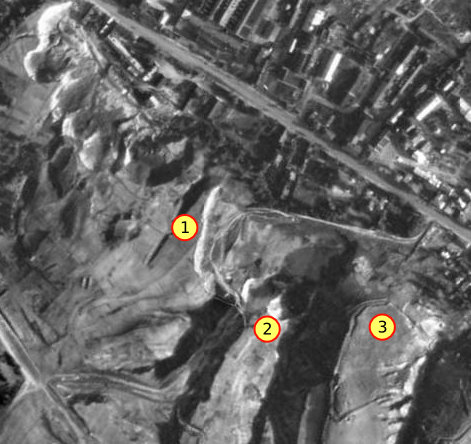
\includegraphics[width=\linewidth]{chast-kirvys/beylis/1943-berner-map.jpg}
\end{center}

Цифрой 1 я обозначил Загоровщину (она простиралась оттуда на северо-запад, по Смородинский спуск включительно). Справа от нее – та самая четкая граница, где теперь оканчивается автобаза. На север от 1, через улицу Кирилловскую, и был завод Бернера (а за ним луг до берега озера Чернечьего), и это его трубы видел Короленко, это его глинища – карьеры – заметны выше и левее от 1, будто огромная челюсть вгрызлась в склон.

Цифрой 2 помечен остаток мыса Кирилловской стоянки. Сейчас он еще более куцый. Под этим мысом было глинище Зайцева. На северо-восток от него – еврейская больница. Видно, что это глинище расползлось на запад до границы 1, и вдоль нее извивается грунтовая дорога, прообраз Богуславского спуска. Вместе с тем граница 1 – это часть широкого, частично срытого мыса Зарембских, затем Бернера. Цифрой 3 я на всякий пожарный отметил мыс с дачами «Кожевника».

То, что называю «огромной челюстью» – как сопоставимо с современным рельефом?  Самый северо-западный надгрыз – закрытый на 2014 год северо-западный въезд на Богуславский спуск, рядом с Кирилловской, 71\footnote{Примерно 50°28′39.2″N 30°29′01.4″E}. Это там мы с Колей Арестовым поднялись на склон и перлись вдоль забора, установленного по верхней кромке, в поисках пещер из дела Бейлиса. Почти шаг за шагом, вся эта местность снята нами на видео – конечно, в кадр попал заросший деревьями и кустами склон, а не лежащие ниже задворки промзоны, куда нас наверняка бы не пустили, а сквозь ветки задворки не особо просматривались.

Учитывая значительность повреждений склона, можно полагать, что если там и были какие-то пещеры, стоянки первобытных людей, кладбища мамонтов, то их благополучно срыли при добыче глины. Неизвестно также, какая степень «разработки» склона была в 1911 году – напомню, мы рассматриваем снимок 1943 года, а с той поры много чего могли раскопать и уничтожить. Не знаю, до каких лет просуществовал завод Бернера. На месте усадьбы Зайцева кирпичный завод обозначен на карте того же 1943 года. Ныне там дом на Татарской, 26-Б.

В материалах по делу Бейлиса, относительно года 1911 пристав Вышинский дает отвечает на вопрос, почему ежели труп был найден в Плоском участке, розыски начала полиция Лукьяновского участка:

\begin{quotation}
У нас в практике так установилось, что если усадьба выходит на улицу Верхне-Юрковскую и если есть постройки, то постройки, которые есть на улицу, входят в лукьяновский участок, а те постройки которые выходят к оврагу, относятся к плоскому участку. Но так как усадьба Бернера никаких построек не имеет, то это относится к участку плоского.
\end{quotation}

%И всюду усадьба Бернера описывается как безлюдная местность.

\newpage

% Как же быть с кожевенным заводом Зарембских? Остался рядом, на Кирилловской 69? Не знаю.

Фотографии из газеты «Киевская мысль» 1911 года, с подписями «Вход в пещеру» и «Труп убитого мальчика».

\begin{center}
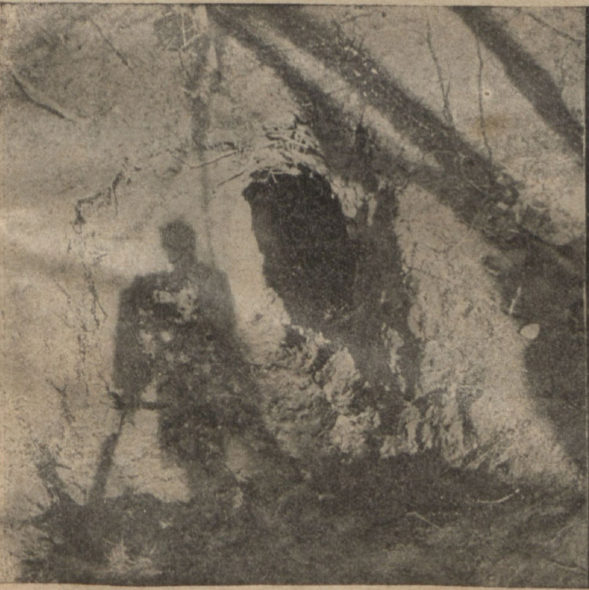
\includegraphics[width=0.85\linewidth]{chast-kirvys/beylis/1911-by-01.jpg}
\end{center}

\begin{center}
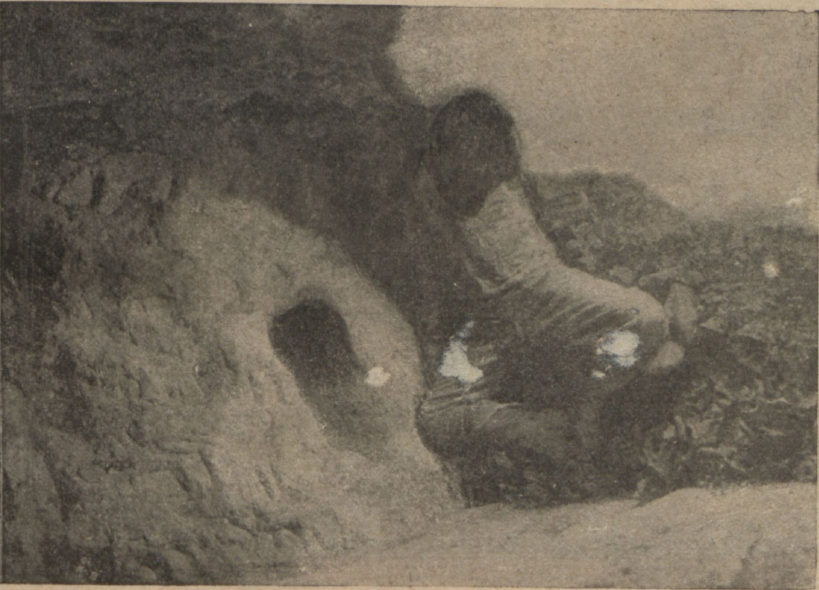
\includegraphics[width=0.85\linewidth]{chast-kirvys/beylis/1911-by-02.jpg}
\end{center}

\newpage

Снимки 1911-го – верхняя часть завода Зайцева и дом Веры Чеберяк:
\vspace*{\fill}
\begin{center}
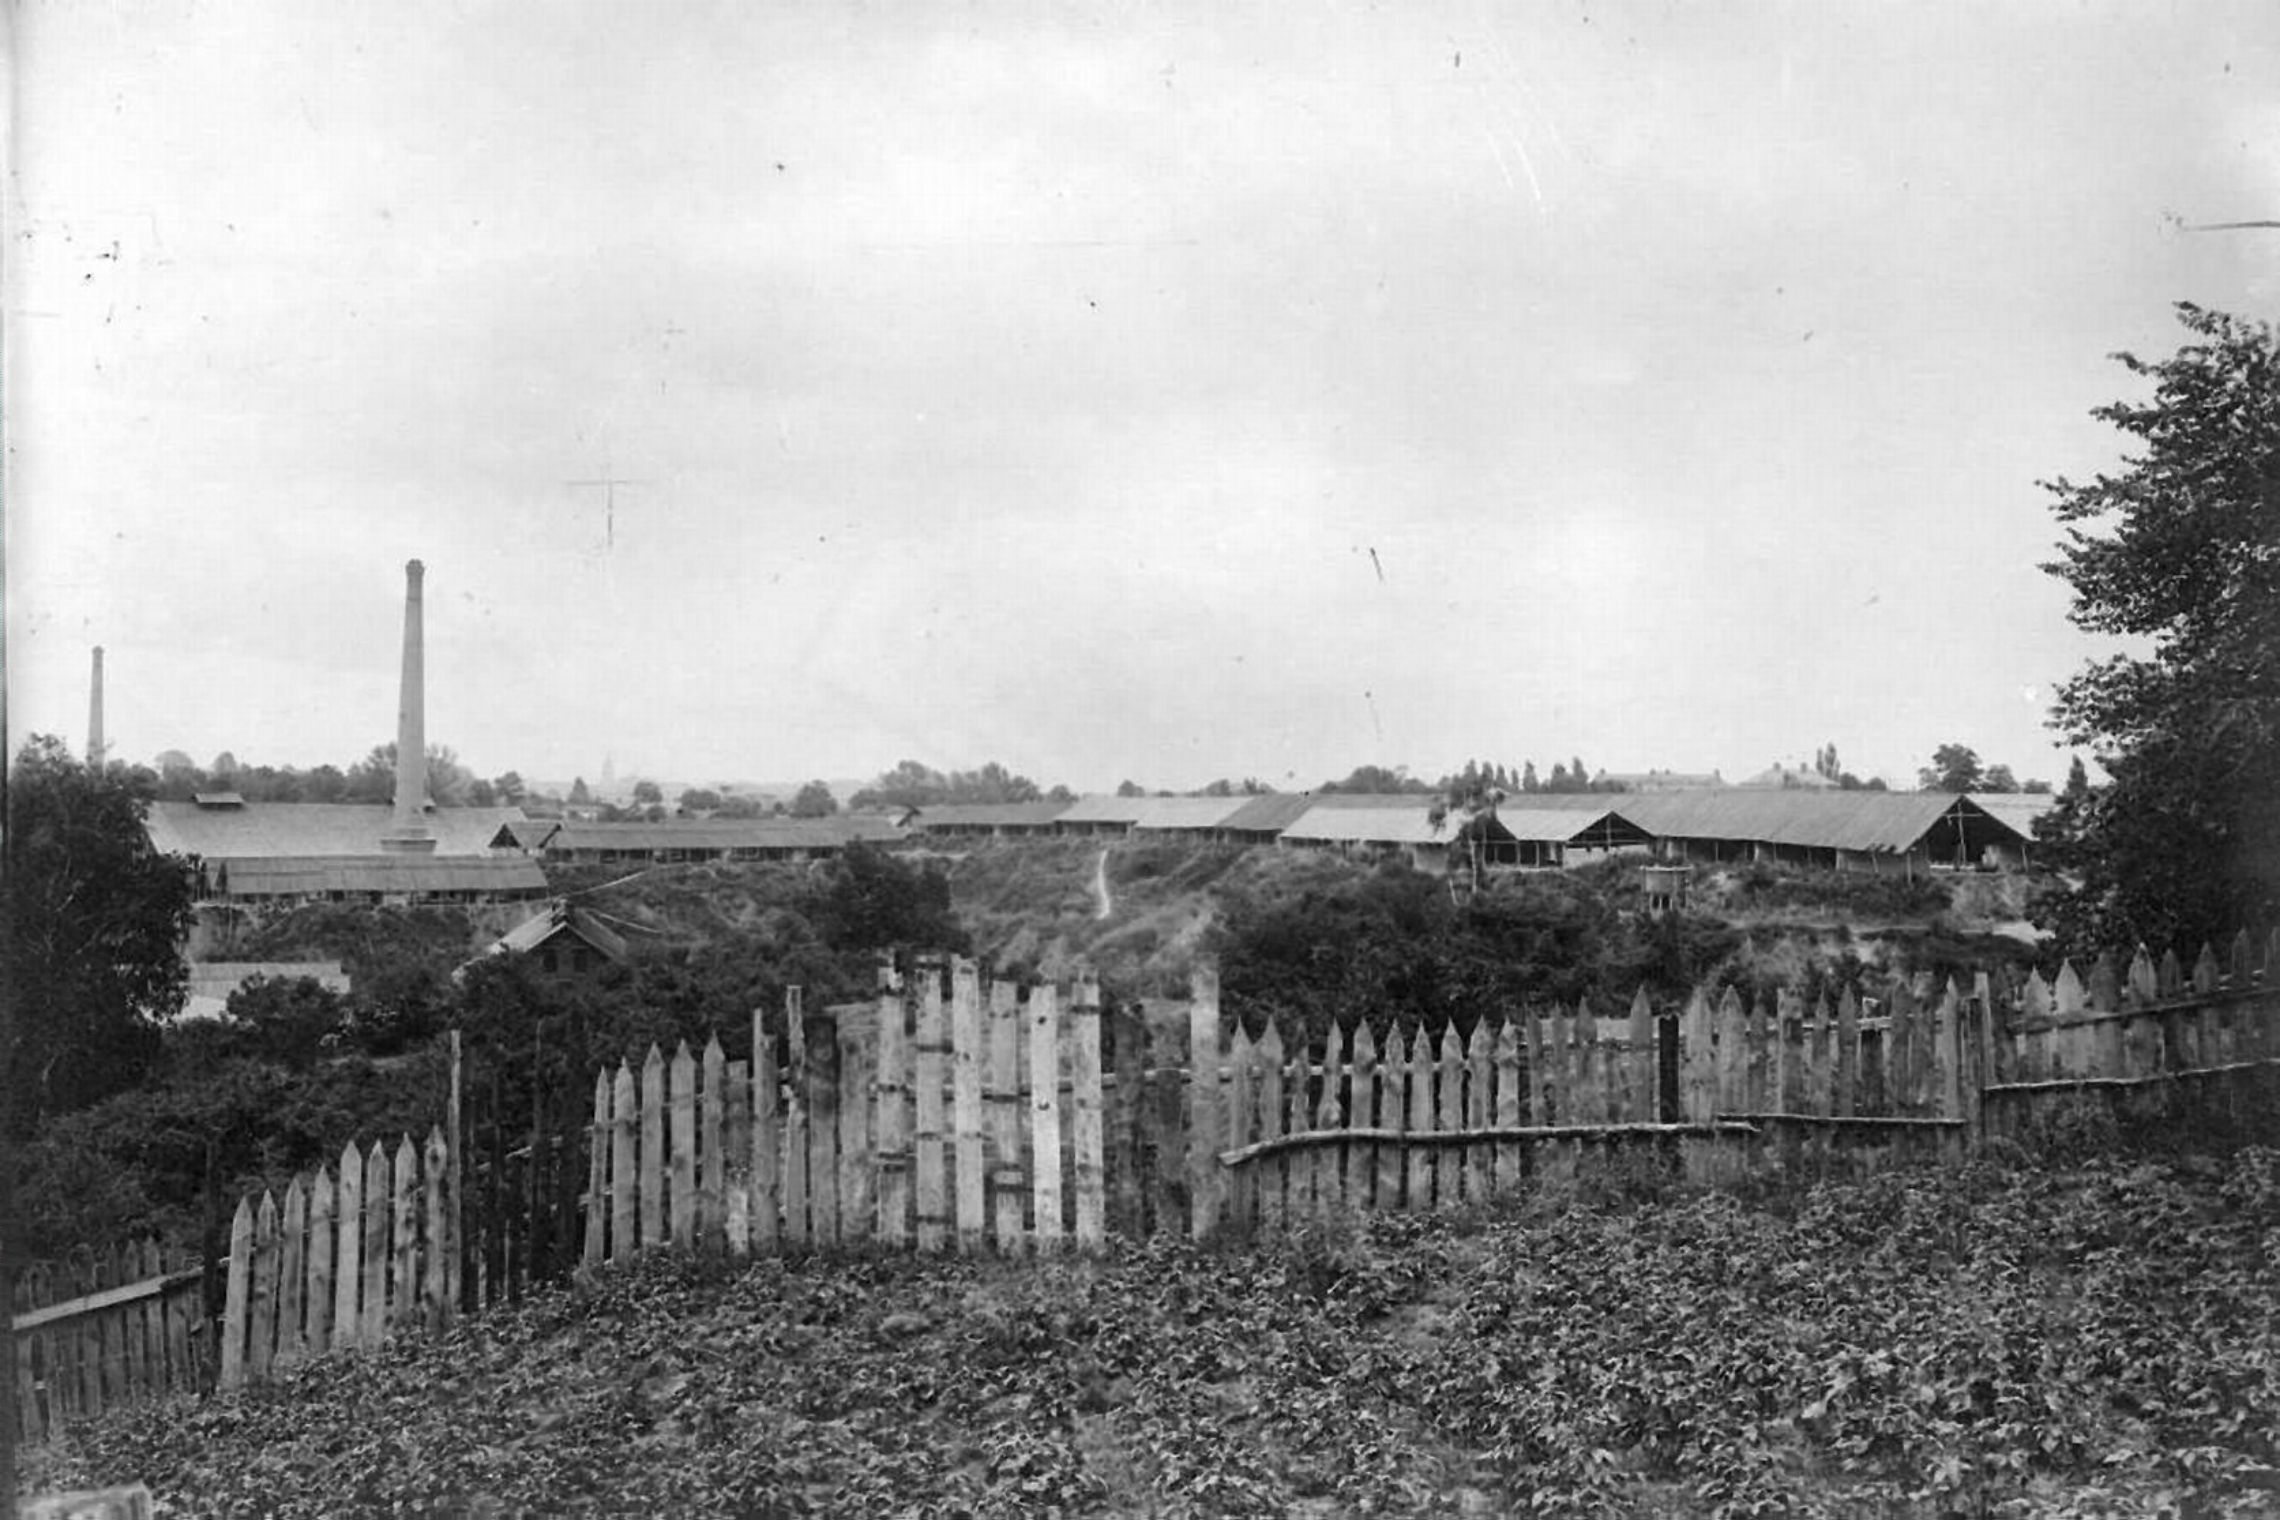
\includegraphics[width=\linewidth]{chast-kirvys/beylis/1911.jpg}
\end{center}

\begin{center}
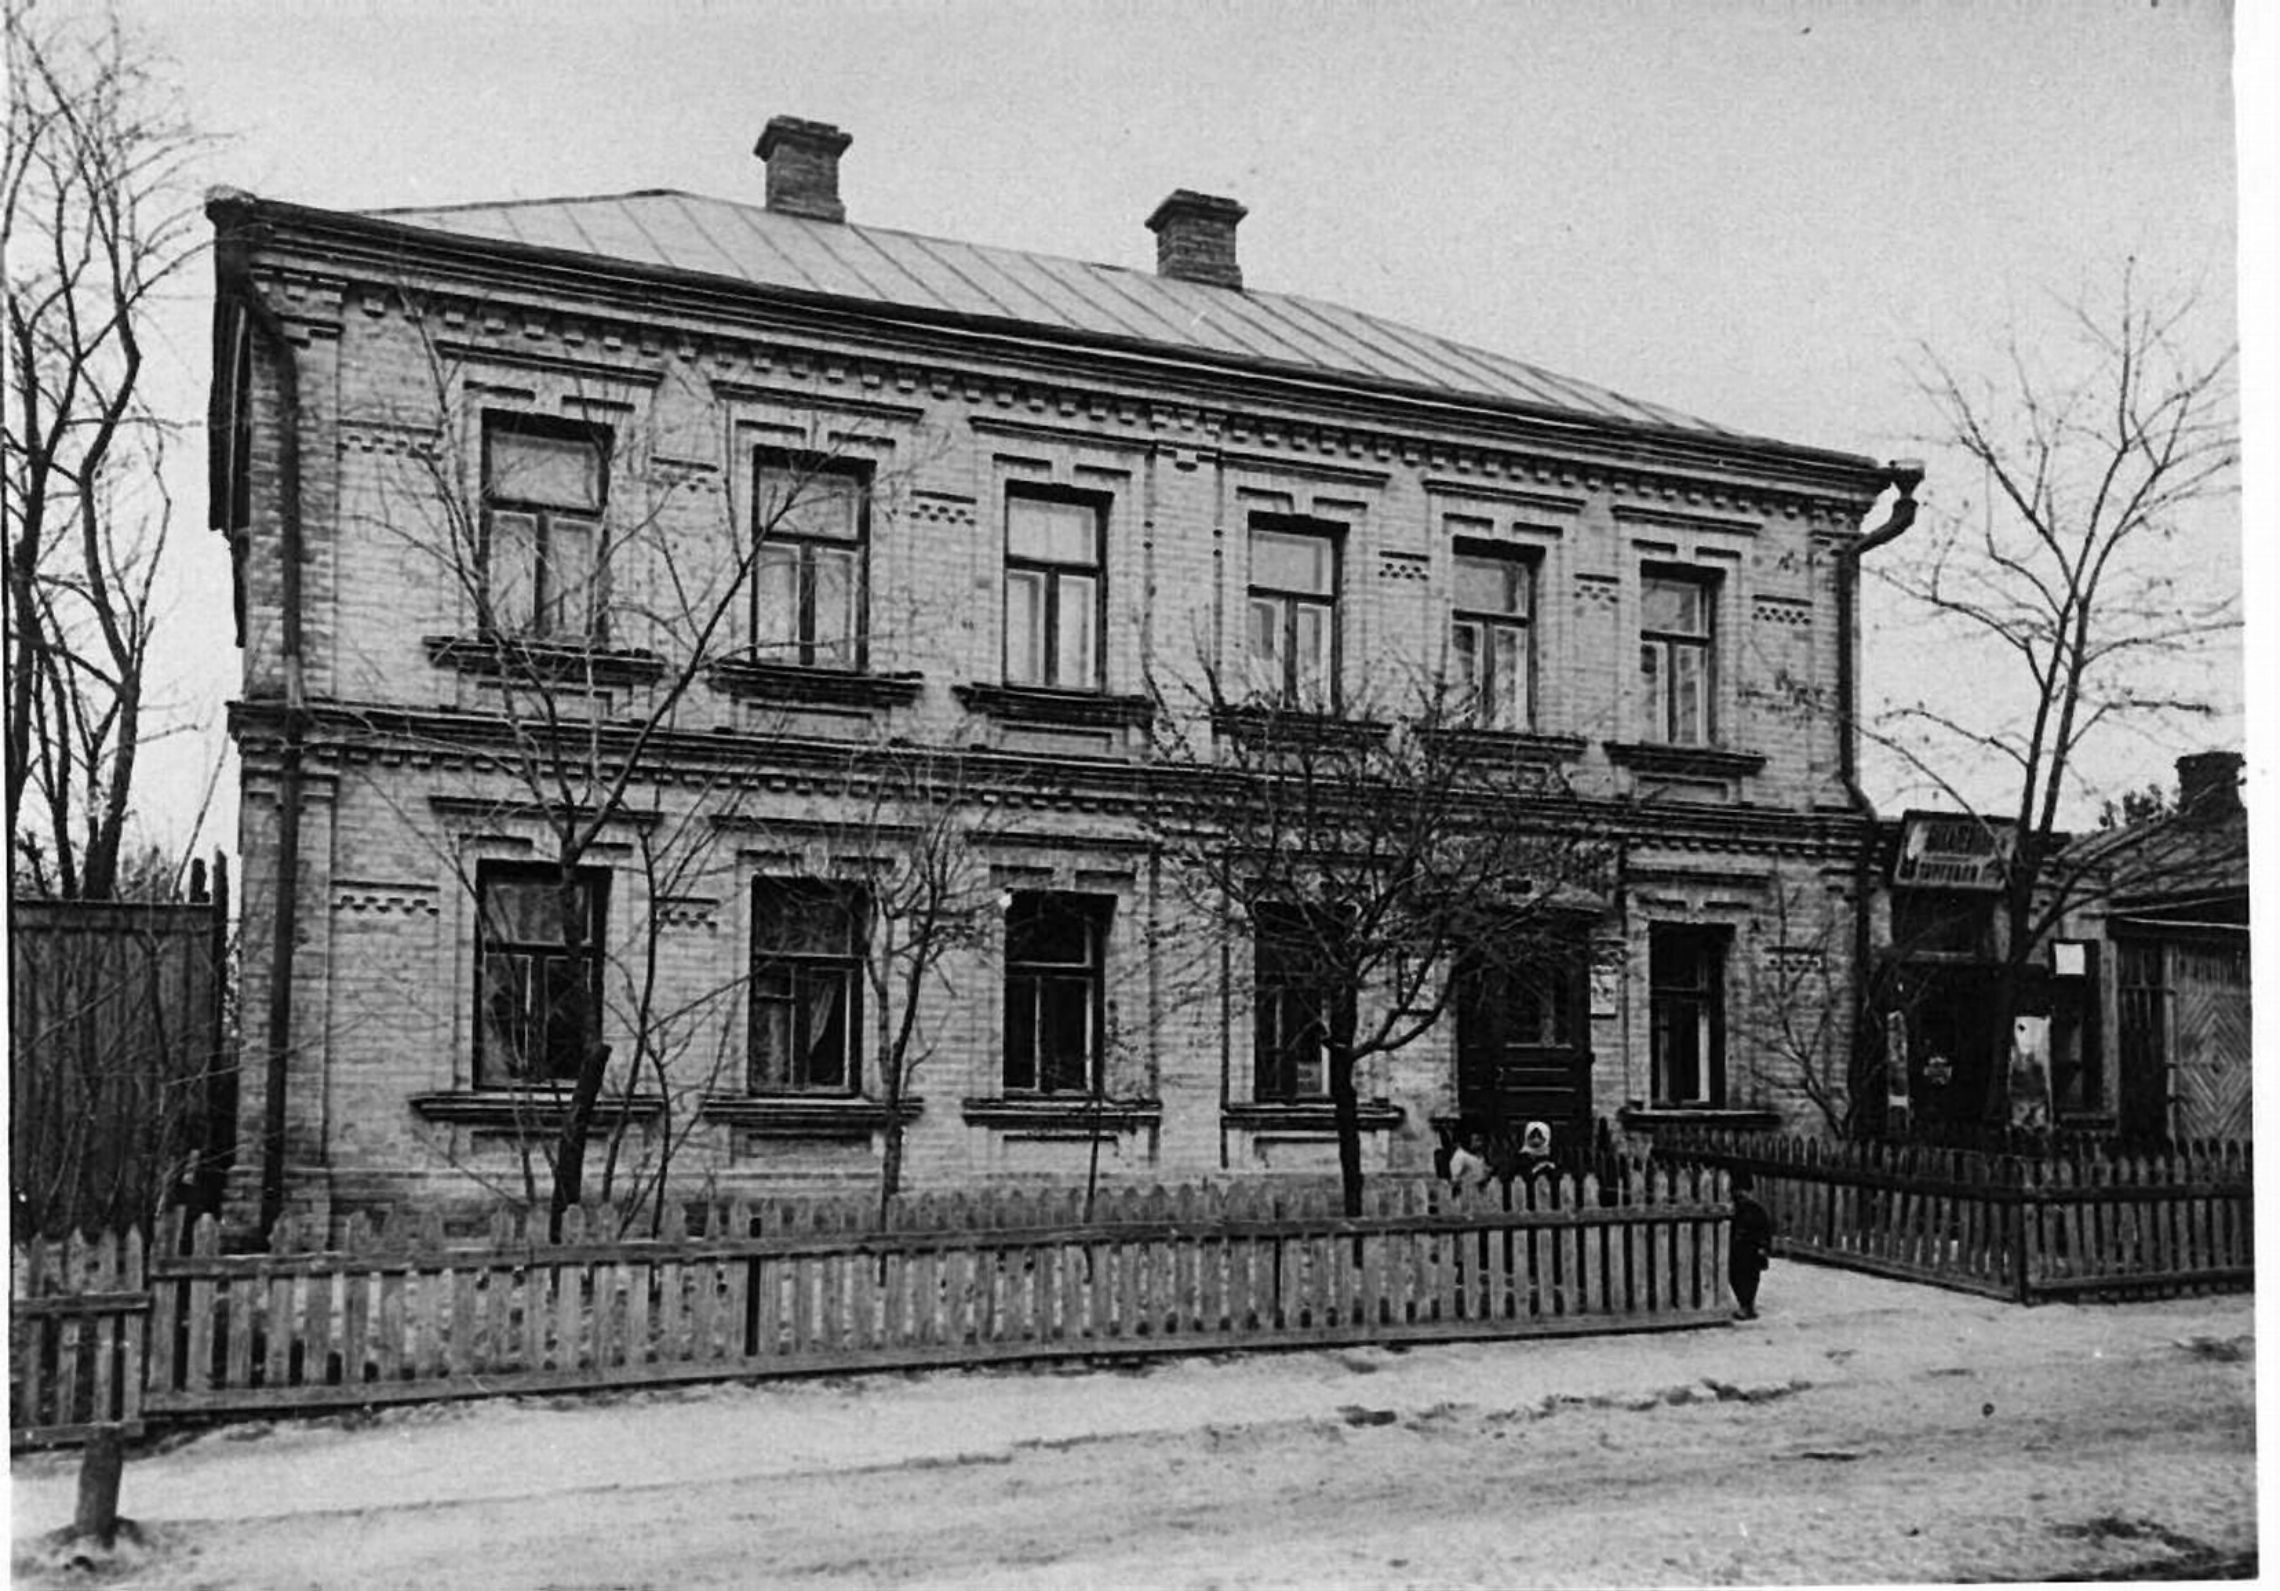
\includegraphics[width=\linewidth]{chast-kirvys/beylis/domcheber.jpg}
\end{center}
\vspace*{\fill}
\newpage


Газета «Киевлянин» за 21 марта 1911 года сообщала:

\begin{quotation}
Убийство. Вчера, 20 марта, около 1 часа дня, гимназист Борис Беломницкий и Петр Эланский, играя в роще, находящейся при усадьбе кирпичного завода Бернера по Кирилловской улице, в районе Плоскаго участка, случайно нашли в небольшой пещере труп мальчика, по виду 10-12 лет, около которого лежал кожанный ученический пояс, несколько тетрадок, фуражка и куртка.

Труп в одном нижнем белье, в неестественном полусогнутом полусидячем положении, был прислонен к стенке пещеры. На голове убитого ясна видна рана, нанесенная, повидимому, каким-то тупым предметом, возможно, что камнем. Руки скручены и связаны на спине. [...]

%Пещера, в которой найден труп, имеет в диаметре более аршина. На глубине ея около сажени, где был труп, она разделяется на два хода. [...]
\end{quotation}

В деле почти не всплывает кирпичный завод Бернера, всё усадьба да усадьба, заброшенный пустырь. Ведь сам завод был по другую сторону улицы, на Кирилловской 88, а склон – это 71.

% Да и усадьбе Бернера в деле мало отводится, и другим пещерам тоже – мол, группа пещер, и всё. То же и Хвойка – отметил курганы, пещеры, и не более того. Во всяком случае, я не знаю его исследований на сей счет.

Вернемся к Короленко. Полагаю, что именно так, как он описывал, мы с Арестовым и поднялись от памятного креста к улице Нагорной. Свидетельство Короленко о пещере можно трактовать по-разному. 

Первое – «холмик» это курган. Ибо Короленко по пути к «той пещере» встретил еще один курган, тоже со входом в пещеру. Стало быть, по крайней мере «та пещера» могла быть вырыта кладоискателями в кургане. 

И другая трактовка – пещеры древние, а курганы не курганы похоронные, а просто бугры, в которых были входы в пещеры.

Давайте поглядим на два снимка входа в пещеру, где нашли тело Ющинского. Их ошибочно помещают как иллюстрацию к раскопкам Антоновича в районе нынешнего Смородинского спуска.

Первый снимок сделан, кажется, раньше второго, ибо нет еще пня, заметного слева над входом в пещеру.

\newpage
\vspace*{\fill}
\begin{center}
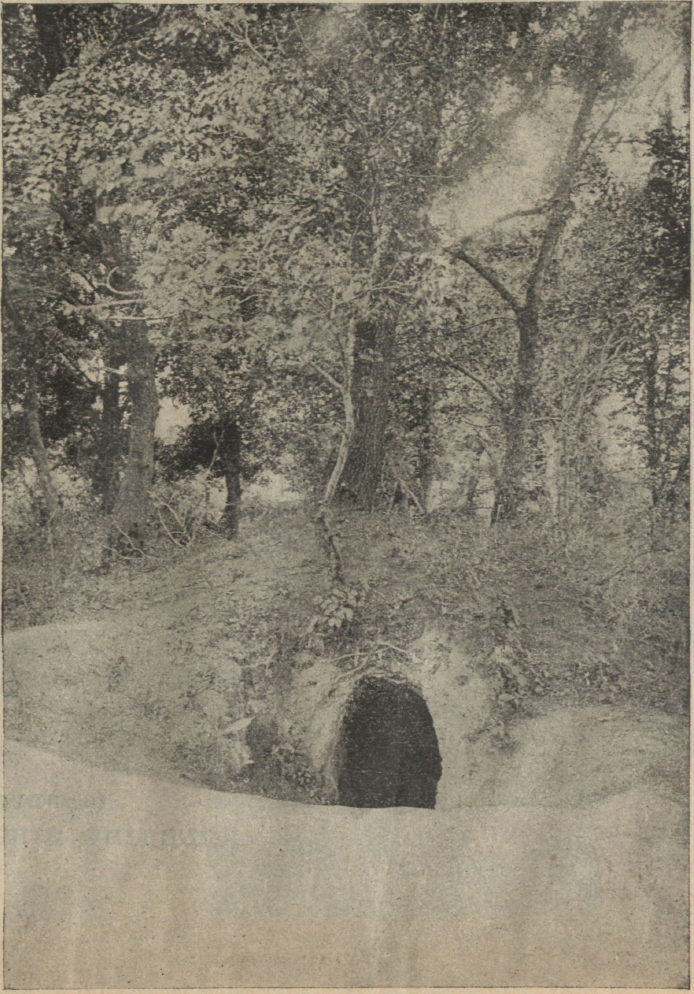
\includegraphics[width=\linewidth]{chast-kirvys/beylis/1912-beylis-01.jpg}
\end{center}
\vspace*{\fill}
\newpage

\begin{center}
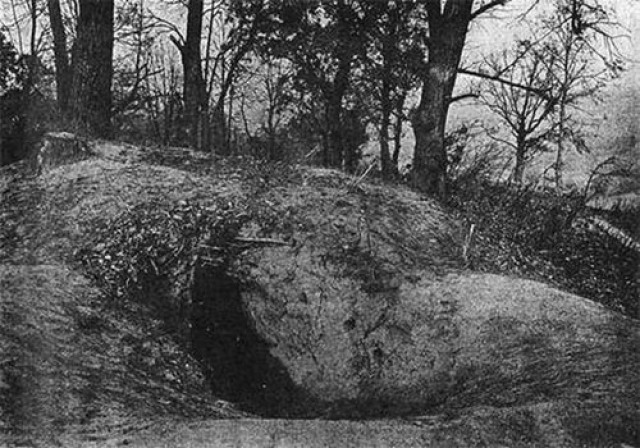
\includegraphics[width=\linewidth]{chast-kirvys/beylis/beylis-peshera-02.jpg}
\end{center}

А на втором можно разобрать окружающую местность. Возвышенность – слева, а понижение склона, «берег» – справа. Такой снимок на Кирилловских высотах можно сделать только стоя на северо-восточном склоне и глядя на северо-запад, либо оттуда же на северо-восток (перпендикулярно Кирилловской улице), ежели находишься на каком-то отроге у основания оного.

Всё это хорошо, но как добраться до этого пятачка? Есть ли дополнительные источники про окружающую местность?

В 1912 году фирма «Пате» сняла документальную хронику (ее можно скачать на \href{http://semiletov.org/kievograd/}{Киевограде} и посмотреть в Ютубе), где перед объективом камеры предстают действующие лица судебного процесса, и разные места. Дом Бейлиса, Чеберяк, завод Зайцева в ложбине, наконец панорама части склона с пещерой – опять же, без привязки к окрестностям. За деревьями ничего не разглядеть, но мы теперь хотя бы знаем, как выглядели ближайшие десять метров около входа!

Я склеил три кадра в один и отметил красным яму со входом в пещеру.

\begin{center}
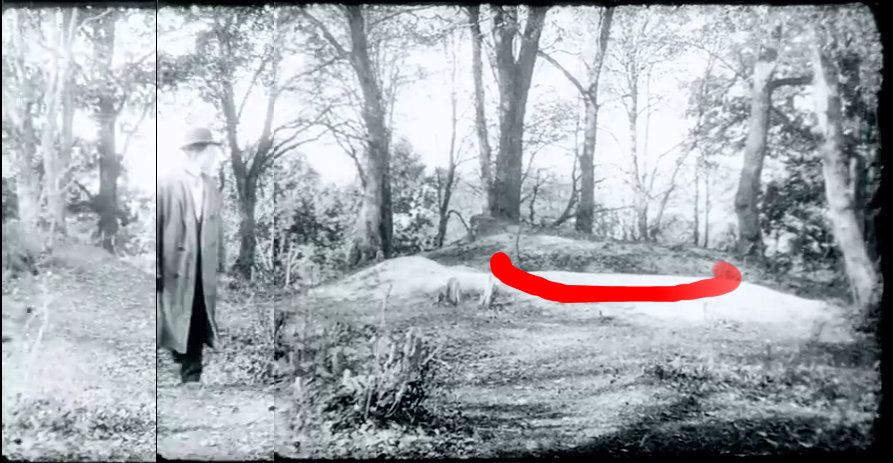
\includegraphics[width=\linewidth]{chast-kirvys/beylis/pesh-comp.jpg}
\end{center}

Что это прояснит в 21 веке? Поглядим еще на отдельный кадр со входом, из той же хроники:

\begin{center}
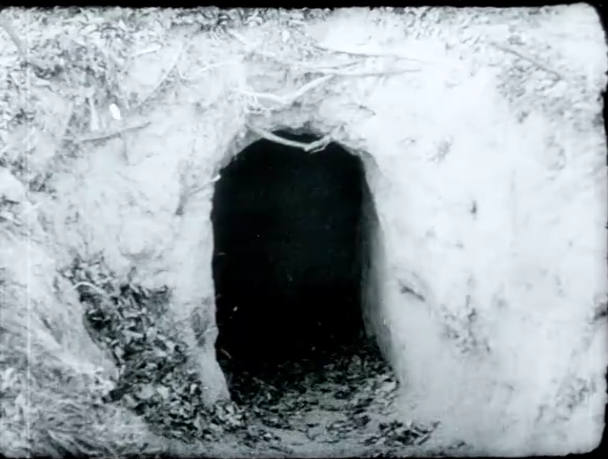
\includegraphics[width=\linewidth]{chast-kirvys/beylis/vhod.jpg}
\end{center}

Итак, яма глубины достаточной, дабы скрыть стоящего взрослого человека. В ее стене такой аккуратный проем 1,06 метра высотой, ведущий в пещеру.

Но давайте попробуем уточнить положение пещеры. 

В стенограммах слушания дела Бейлиса есть следующие показания свидетеля Эланского о местности и пещере, где нашли труп:

\begin{quotation}
Председатель: Объясните нам, место, о котором вы говорили – не любимое ли место, где гуляют мальчики?

Эланский: Да, любимое.

Председатель: Там много пещер?

Эланский: Да.

Председатель: В этом месте нет построек, гулять там можно свободно? играть в снежки, шалить? вас никто не останавливает?

Эланский: Да.

Председатель: Там улица есть?

Эланский: Якубенковская улица.

Прокурор: Она выходит на Нагорную улицу? А пещера недалеко от Нагорной улицы?

Эланский: Недалеко.

Председатель: Якубенковский переулок выходит на Нагорную улицу. В течении какого времени пройти можно от пещеры до этой улицы? Минуты три достаточно?

Эланский: Не знаю, может быть, это недалеко.

Председатель: Если быстро идти, минуты три достаточно?

Эланский: Да.
\end{quotation}

Якубенковская улица нынче носит имя Тропинина, но та часть её, что пересекала Нагорную в сторону склона холма и Кирилловской, была в 1938 году отчекрыжена и переименована в переулок Репина. Эту-то часть и упоминает топографически Эланский, говоря о Якубенковской улице. 

Напрасно искать на карте переулок Репина! В 1952 году его переименовали в Нагорный тупик, а в 1980 – устранили вовсе и место тупика занял построенный к Олимпиаде гостинично-спортивный комплекс «Авангард» по адресам улица Нагорная, 25-27. На 2021 год это уже не «Авангард», а офисный центр ООО «Славянский дом ФПУ» (учредитель – Федерация профсоюзов Украины).

Между ним и автобазой и лежит местность, где, по всем прикидкам, раньше были пещеры и среди них та, в которой нашли тело Ющинского. На склоне, начиная от Нагорного переулка, и далее на юго-запад и до памятного креста – пещер нет, мы с Колей Арестовым там всё облазили – уточню, от забора и вниз. За забором в сторону Татарки мы не смотрели. Мы лезли вдоль забора по кромке обрыва и осматривали склон. А если подниматься от памятного креста в сторону Нагорной – тоже пещер не нашли, включая овраг к юго-востоку от бывшего «Авангарда». Впрочем среди зарослей порой сложно что-либо рассмотреть.

В первом томе материалов из суда по делу Бейлиса, на странице 212 приведен следующий протокол осмотра пещеры:

\begin{quotation} 
Протокол №1. 1911 года, марта 21 дня. И.Д. судебного следователя, 5 уч. г. Киева, получив сообщение пристава плоскаго, города Киева, участка, от 20 марта, 1911 года, за №11710, о найденном в усадьбе Бернера, по Кирилловской улице, труп убитого ученика киево-софи\-йского духовного училища Андрея Ющинского, немедленно прибыл на место нахождения трупа, в присутствии ниже поименованных понятых, производил осмотр трупа и окружающей местности, причем оказалось: труп Андрея Ющинского  находился в усадьбе Бернера, на Кирилловской улице, под №71. 

Усадьба эта представляет собою обширную, в неск\-олько десятин, гористую, в верхней своей части пустопорожнюю усадьбу, фронтом выходящую на Лукьяновке. Переднюю часть усадьбы со стороны Кирилловской улицы занимает глинище, где добывается глина для кирпичного завода Бернера, находящегося в усадьбе его по Кирилловской улице, №88, а задняя часть усадьбы представляет собой вершину крутой горы, с разбросанными по ней буграми, рытвинами и ярами, и покрытую крупным лиственным лесом и кустарником.

Усадьба эта ни от Нагорной улицы, ни от соседних с ней усадеб, имеющий такой же пустынный, гористый и лесистый характер, не огорожена, но по ней во многих местах проходят тропинки в разных направлениях.

Место, где найден труп Андрея Ющинского, находится в верхней части означенной усадьбы и в расстоянии около 15 сажень\footnote{32 метра.}, от Нагорной улицы и в расстоянии около версты от Кирилловской.

Выступ к месту нахождения трупа со стороны Кирилловской улицы очень затруднительный, вследствие крутизны подъема, с Нагорной ул., совершенно свободный.

Ближайшие жилые постройки к месту нахождения трупа виднеются в расстоянии около полуверсты\footnote{Около 530 метров.}.

Труп Андрея Ющинского находится в пещере, вырытой в небольшом кургане, покрытом по краям крупными деревьями. 

При прибытии судебного следователя, вокруг этой пещеры, охраняемой полицией, стояла густая толпа народа. К входу в пещеру ведет довольно крутой, сажени полторы длиною\footnote{3,2 метра.}, спуск, покрытый грязью и засохшими листьями.

Вход в пещеру, обращенный на юг, имеет около 1 аршина ширины, и около полутора аршина высоты\footnote{Ширина около 71 см, высота примерно 106 см.}, так что проникнуть туда взрослому человеку, можно только согнувшись, но в глубине пещеры высота ее доходит до двух с четвертью аршин, а ширина до 1 с 1/4 аршина\footnote{В глубине высота до 160 см., ширина до 80 см.}. Длина этой пещеры, попрямому направлению около 4 аршин\footnote{2,28 метра.}.

На расстоянии 2 с 1/2 аршин\footnote{175 см.} входа с левой стороны имеется разветвление пещеры, поворачивающее под прямым углом влево, и имеющее около одного аршина ширины, около 1 1/2 аршина длины, и около 2 1/4 аршина высоты\footnote{Ширина 71 см., длина 106 см., высота 160 см.}, в каковом разветвлении пещеры и лежит труп Андрея Ющинского.

На расстоянии около 3 арш.\footnote{213 см.} от входа в пещеру, с правой стороны имеется второе разветвление пещеры, поворачивающее под прямым углом вправо, и имеющее в ширину около одного аршина, в высоту около 1 1/2 аршина, и в длину около 2 3/4 аршина\footnote{Высота 106 см, длина 196 см.}. В этом разветвлении найден кусок порванной смятой газеты со следом крови.

Труп лежит в согнутом положении, и упирается верхней частью спины и головой в заднюю стенку левого разветвления пещеры, а ногами в переднюю стенку того же разветвления. Голова несколько наклонена вниз и вбок, к выходу из этого разветвления пещеры, ноги раздвинуты в бедрах, и подошвами касаются она другой, правая нога в суконном красном с синими полосками чулке, с порванными пяткой и носком. На чулке этом, возле колена, имеется развязанная подвязка в виде тесемки, левая нога голая, обе руки подогнуты под спину и у кистей туго связаны шпагатом, под трупом лежит довольно много сухих листьев, в также найден кусок смятой газеты «Южная копейка» №1, от 1-го января, 1911 года. 

В боковой стенке этого разветвления пещеры, на высоте 1/2 аршина\footnote{35 см.}, от дна ея имеется печурка длиною около аршина и глубиной и высотой около полурашина\footnote{35 см.} и глубиной и высотой ки пещеры\footnote{«ки пещеры» – так в источнике.} найден красный с синими полосками суконный чулок, очевидно снятый с левой ноги покойного.

Лицо покойного окровавлено и выпачкано в глину, на голове также заметные следы крови и глины. Ворот рубахи расстегнут, кальсоны расстегнуты и немного спущены.

Затем труп для дальнейшего осмотра был извлечен из пещеры. Одет он был только в серо с синими продольными полосками кальсоны, и нижнюю холщовую рубаху с вышитым в крестик воротом, грудью, обшлагами рукавов и подолом. На шее, в области сердца, на правом боку и на спине трупа замечаются многочисленные, небольшие колотые раны, причиненные острым колючим орудием, вроде шила. Подштанники в верхней своей части окровавлены и местами окапаны стеарином, рубаха также окровавлена, преимущественно на груди, на голых ягодицах замечаются следы желтой глины и сухих листьев. Тужурка, картуз, пояс и тетрадка покойного, найденные по объяснению присутствовавшего при осмотре помощника пристава плоского города Киева участка, Вышинского, в пещере возле трупа, взяты были к дознанию до прибытия судебного следователя.

В пещере нигде на земле следов крови не обнаружено. Почва дна пещеры – рыхлая желтая глина, перемешанная с сухими листьями. Осмотр пещеры произведен был при свете фонаря. Судя по тесноте пещеры и по отсутствию следов крови, на дне пещеры, надо полагать, что покойный был лишен жизни не в этой пещере, а где-нибудь в другом месте. Никаких других следов преступления ни в пещере, ни в окружающей местности не обнаружено. 

Осмотренная пещера имеет следующий вид.

А. Вход в пещеру. Б. Левое разветвление пещеры, и место нахождения трупа Андрея Ющинского. В. Правое разветвление пещеры.

Засим было сделано распоряжение о доставлении трупа в анатомический театр университета св. Владимира, для судебно-медицинского осмотра и вскрытия. Найденные при осмотрел два куска газеты и чулок, взяты к делу. И.д. судебного следователя (подпись). При осмотре понятыми были городовой плоского участка Иван Васильевич Крименко и мещ. Моисей Павлович Гасан.
\end{quotation}

А вот из того же тома материалов, протокол осмотра усадьбы:

\begin{quotation} 
13 октября суд. след. киевск. окр. суд. по особо важным делам В.И. Фененко в присутствии тов. прок. киевск. окр. суда. Е. И. Лашкарева и нижеподписавшихся понятых, производил осмотр усадьбы, в которой находится кирпичный завод Зайцева и дополнительный осмотр (лист 8 и 230, т.1) прилегающей к местности, причем оказалось следующее:

Осматриваемая усадьба имеет около 10 дес. земли, окружена высоким дощатым забором и не везде исправным и выходит на Кирилловскую ул., где значится под №16\footnote{Очевидная ошибка, усадьба Бернера имеет номер 71, рядом смежные номера, к тому же речь идет о нечетной стороне Кирилловской улицы.}, по В.-Юрков\-ской ул., где значится под №32, и на Нагорную ул., без обозначения номера.

На каждой из этих улиц выходят из усадьбы Зайцева ворота. И с левой стороны ворот, ведущих на Нагорную ул., к усадьбе Зайцева отгорожен небольшой кусок земли, составляющий ныне усадьбу Богдановского. Здесь находятся изба его и сарайчики. 

Из усадьбы Богдановского на Нагорную ул. в усадьбу ведет дорога, имеющая незначительный уклон внутрь усадьбы. 

С правой стороны от дороги, а также выше над откосом расположен целый ряд навесов для сушки кирпича, между которыми имеется несколько кругов «мял» для вымешивания глины.

С левой стороны от дороги в расстоянии 162 шагов от входных в усадьбу ворот, находится небольшой необитаемый ныне дом, в котором проживает свидетель Юхриков.

В расстоянии 65 шагов от этого дома расположен круг, «мяло» для вымешивания глины, а от этого места на расстоянии 40 шагов выстроена кирпичеобжигательная печь, носящая название нижней печи. Эта обжигательная печь представляет собой кирпичное здание овальной формы. В деревянном чердачном помещении этого здания имеется целый ряд тюков, для бросания в них дров, само же здание имеет 16 входов для нагрузки кирпича.

Кроме обжигательной печи выстроен деревянный навес, крыша которого соединяется с крышей печи; под навесом складывается обожженный кирпич. Длина печи по навесу 66, а ширина 28 шагов.

От описанного выше мяла до дымогарной заводской трубы ведет дорога на расстоянии от печи 120 шагов, а затем тропинка по косогору вверх на расстоянии 90 шагов, т.е. всего на расстоянии 210 шагов.

От дымогарной трубы в расстоянии 20 шагов выстроена вторая кирпичеобжигательная печь, носящая наименование верхней печи такой же формы, величины и устройства, как и нижняя печь.

Во время осмотра обе печи оказались загруженными кирпичом и поэтому не представляют возможным подробно осмотреть их. Ознакомиться же на месте с устройством их, по объяснению лица заведывающего обжиганием кирпича, также было невозможно, в виду временного отсутствия того лица, вследствие подробный осмотр печи отложен на другой срок.

С левой стороны от верхней печи по направлению к Кирилловской ул. выстроен целый ряд навесов для сушки кирпича, а далее в том же направлении, у обрыва, в расстоянии 230 шагов от дымогарной трубы была выстроена конюшня, имевшая 60 шаг. длины и 15 шаг. ширины. Под одной крышей с этой конюшней имелось небольшое жилое помещение, в котором находилось, по объяснению присутствовавших по осмотре рабочего Харитона Быковца, шорная мастерская где были найдены приставом Красовским швайки, приобщенные к делу в качестве вещественных доказательств.

Во время осмотра строения, в котором помещалась конюшня и вышеозначенное жилое помещение, а также и соседний навес для сушки кирпича оказались уничтоженными пожаром, бывшим 10 октября, причем от конюшни и навеса осталась груда обгоревших бревен, от жилого же помещения сохранились отчасти стены.

За местом, где была конюшня, идут откосы, и ниже их, по высокому обрыву, имеется глинище, с выстроенной над ним водокачкой.

Мимо этого глинища дорога спускается вниз к воротам усадьбы, выходящим на Кирилловскую ул. 

Недалеко от ворот, с левой стороны от дороги, находятся два деревянных, одноэтажных дома, в одном из которых помещается еврейская богадельня, а несколько ниже несовсем оконченный постройкой деревянный дом, выходящий на Кирилловскую ул.

По показанию присутствовавшего при осмотре помощника пристава плоского участка Вышинского, дворницкая, где помещалась шорная мастерская, а также и сарай снесены нес\-колько месяцев тому назад. Место, где они находились, оказалось у обрыва.

Ниже этого обрыва недалеко от забора, отделяющего усадьбу от Кирилловской ул., выстроено вчерне каменное двухэтажное здание для больницы, а рядом с ним расположено старое больничное здание.

От дымогарной трубы мимо верхнеобжигательной печи, по направлению к В.-Юрковской ул., несколько в гору идет дорога к воротам, выходящим на эту улицу. Расстояние по дороге от верхней печи до В.-Юрко\-вской ул. – 180 шагов.

Справа и слева от этой дороги расположены навесы для сушки кирпича, а у входных ворот на В.-Юрко\-вскую ул. выстроен одноэтажный с деревянным помещением дом, в котором проживал заводской приказчик\footnote{По некоторым данным, Бейлис не состоял приказчиком, однако выполнял на заводе присущую этой должности работу.} Мендель Бейлис и помещалась заводская контора.

Усадьба И. Зайцева по В.-Юрковской ул. имеет 64 шага длины. В 12 шагах от угла усадьбы Зайцева по В.-Юрковской ул. имеется водоразборная будка городского водопровода. Присутствовавший мальчик Константин Добжанский указал на это место, где он видел Андрея Ющинского дней 10 до обнаружения его трупа. Место это находится возле водозаборной будки. По объяснению Добжанского, Ющинский, перейдя отсюда на другую сторону В.-Юрков\-ской ул., пошел по ней по направлению к Печенеговской ул. 

Место, куда пошел Ющинский, пока его видел Добжанский, находится на расстоянии 70 шаг. от водоразборной будки.

За водопроводом по направлению к Половецкой ул. расположены усадьбы частных владельцев, граничащие с заводской усадьбой Зайцева и отделяющиеся от ее высоким дощатым забором. Среди этих усадеб расположена усадьба Захарченко, значащаяся по В.-Юрковской под №40 и имеющая по В.-Юрко\-вской ул. 25 шаг. длины. В этой усадьбе проживала с семьей свидетельница Вера Чеберякова. Дом, во 2-ом этаже которого жила названная Чеберякова, двухэтажный, выходит в фасад на В.-Юрковс\-кую.

Кроме двухэтажного дома в усадьбе Захарченко расположены сарай и флигель. От входных в усадьбу ворот до забора, отделяющего усадьбу Захарченко от усадьбы Зайцева, 105 шагов. В глубине этой усадьбы в саду, в расстоянии 11 шаг. от старого полуразрушенного забора, отделяющего Половецкую ул. от усадьбы Захарченко, стоит небольшая изба. 

На углу В.-Юрковской и по Половецкой ул. находится усадьба Шаховской, имеющая по В.-Юрковской 31 шаг и по Половецкой ул. 44 шага длины. Здесь на углу этой усадьбы, по показанию присутствовавшей при осмотре свидетельницы Ульяны Шаховской, она увидела 12 марта Андрея Ющинского и Женю Чеберяка.

За усадьбой Шаховской по Половской ул. под №1 расположена усадьба Петренко, имеющая в длину по улице 38 шагов. От угла В.-Юр\-ковской ул. до начала Нагорной ул. 114 шагов.

Нагорная улица без построек вначале, глухая, имеет с правой стороны, если идти с Половецкой ул. по направлению к Ново-Богоутовс\-кой ул. заборы заводской усадьбы Зайцева, а с левой стороны – березовую рощу усадьбы Истомина.

От начала Нагорной ул. до входных в усадьбу Зайцева ворот – 180 шагов. Ворота имеют 9 шагов ширины. От ворот до калитки, ведущей с Нагорной ул. в усадьбу Богдановского, 38 шагов, а от калитки до угла этой усадьбы 5 шагов.

Далее по Нагорной улице широкое открытое место, по которому идет дорога к Якубенковскому переулку. В нескольких шагах от дороги с правой стороны имеется канава, глубиной в нескольких местах около двух, а в других около трех аршин. От ворот, ведущих в усадьбу Зайцева до начала канавы 105 шагов.

Василий Ященко из этой канавы увидел 12 марта сего года незнакомого ему человеку, шедшего по направлению к урочищу «Загоровщина». Место канавы, где по указанию Вышинского свидетель Ященко остановился для отправления естественной надобности, находится от начала канавы в расстоянии 28 шагов, и в 30 шагах по прямой линии от границы усадьбы Лубенского. Второе место за канавой, где по указанию Вышинского свидетель Ященко, увидя незнакомца, остановился и пробежал некоторое расстояние, находится в 110 шагах от первого места. От этого последнего места до того места, где незнакомец остановился и посмотрел на свидетеля Ященко, по прямой линии 94 шага.

От места, где остановился незнакомец, до начала заросли усадьбы Бернера 36 шагов, и отсюда до пещеры, где был найден труп Андрея Ющинского 54 шага.

Шел незнакомец, как объяснил свидетель Ященко помощнику пристава Вышинскому, сначала по ведущей с Нагорной тропинке, по которой можно дойти до пещеры, но затем остановился. Свернул с тропинки и, заметив свидетеля Ященко, пошел в противоположную сторону от пещеры, где был найден труп Ющинского.

Между усадьбой Бернера, где находится оз\-наченная пещера и усадьбой завода Зайцева расположены усадьбы: 1) наследников Соколовского, 2) Лубенского и 3) Марра. Осмотр их произведен 7 мая сего года, в пещере, где обнаружен был труп Ющинского до ворот усадьбы Зайцева, выходящих на Нагорную улицу, если идти по прямому пути, но, по возможности зарослями, по усадьбе Бернера пересечь поляну Соколовского, идти по этой последней усадьбе до угла ее и затем по Нагорной до ворот усадьбы Зайцева, – 366 шагов. 

Вся осмотренная местность снята на плане, на котором приведены необходимые объяснения.
\end{quotation} 

Из обвинительного акта, раздел «Находка трупа Ющ\-инского»:

\begin{quotation} 
20 марта 1911 года, на окраине города Киева, в покрытой зарослями усадьбе Бернера, выходящей  неотгороженной стороной на Нагорную улицу, вдали от построек, в одной из находящихся там пещер, на расстоянии 150 сажен\footnote{320 метров.} от этой улицы, был обнаружен труп мальчика.
\end{quotation} 

Еще в одном месте упомянуто, что пещера расположена в «леске».

В протоколе описания пещеры написано, что она лежит в 15 саженях (32,4 метра) от Нагорной, в верхней части усадьбы! 32 метра – получается почти на обочине! Это противоречит данным из обвинительного акта и протоколу описания местности.

Там же, в протоколе, есть описание объектов – тех же, что на карте 1913 года, с измерением расстояния между ними в шагах. Нас интересуют объекты, обозначенные на карте номерами 12, 13, 14.

12 – на Нагорной, 14 – пещера. Сложив расстояния между этими объектами, мы получим расстояние от Нагорной до пещеры. 94+36+54=184 шага. Приняв, что шаг равен аршину, вычислим, сколько это будет в метрах. 184*71,12/100=130,861. Итого 131 метр. Это уже реалистичней, нежели 32 метра. Но все равно не похоже на 320 метров из обвинительного протокола. 

На карте, пещеры и глинище Зайцева приблизительно одинаково удалены от населенной местности, и 320 метров примерно соответствует участку склона, где установлен теперь памятный крест. И 320 метров – примерное расстояние от населенной местности до глинища усадьбы Зайцева. 

Так что же, числа, обозначающие расстояния, в протоколе описания пещеры и в протоколе описания местности, для вычисления пещеры в итоге дают ошибку? Если да, то, как я понимаю, пещера с телом Андрей Ющинского, обращенная входом к югу, была на части склона, занимаемого теперь западной частью автобазы (Богуславский спуск, 5). 

Из описания выездного заседания суда («Дело Бейлиса. Стенографический отчет», том 1) можно почерпнуть сведения, как добраться до пещеры сверху, от усадьбы Захарченко (Верхне-Юрковская\footnote{Сейчас улица Отто Шмидта.}, 40):

\begin{quotation}
Но Карабчевский предварительно просит еще раз подойти к усадьбе Захарченко со стороны Нагорной улицы.
 – Вот, – говорит он, обращаясь к присяжным заседателям, – усадьба, в которой раньше жила Чеберяк. Вы видите, господа, что из этой усадьбы ведет прямой тракт по глухой, нежилой и совсем незастроенной улице к пещере, где найден труп.

Уходят и направляются к пещере. По дороге Ященко показывает место, где в день убийства видел человек с черными усами, входящего в лес. В этот лесок, где находится пещера, все и спешат. [...]

Когда осмотрели пещеру, г. Шмаков, показывая на завод Зайцева, говорит:
 – Гг. присяжные заседатели, запомните, что от этого места (вблизи пещеры) до завода Зайцева – прямая линия.
\end{quotation}

Усадьба Захарченко применительно к 2017 году, стояла (уходя вглубь на север) около перекрестка Татарской и Половецкой, с основным зданием эдак примерно напротив современного №33 на Отто Шмидта.

Далее коснусь сведений, которые помещаю в свою книгу неохотно, поскольку изложение их потребует множества пояснений. На первый взгляд слова четкие и ясные становятся противоречивыми, как только перестаешь относиться к ним поверхностно, принимать как есть.

Подзабытое имя зоолога и краеведа Николая Шарлемань (1887-1970) понемногу выходит из тени, его наследие цитируется в качестве источников. Хорошо бы я мог радоваться редким свидетельствам. Да в сравнении высказываний Шарлеманя об одном и том же предмете в разное время обнаруживаю нестыковки, не говоря уже о сравнении с источниками внешними по отношению к Шарлеманю. В некоторых случаях эти нестыковки я бы списал на свое невежество, пробелы в знаниях, однако прочие ставят меня в тупик – как относиться к ним ? 

Шарлемань был свидетелем со стороны защиты Бейлиса, и много лет спустя вспоминал\cite{sharl01}:

\begin{quotation}
В усадьбе Зайцева по Кирилловской улице № 59, где была открыта стоянка людей каменного века, произошло знаменательное событие, которое эту довольно известную усадьбу сделало еще более известной. В те годы я работал в газете «Киевская
мысль», где вел отдел «Наблюдения за природой» и опубликовал разные материалы под рубрикой «Из жизни природы». Местом наблюдения для меня служили холмы, покрытые лесом, по левой стороне Кирилловской улицы. Сюда почти ежедневно я ходил с научной экскурсией, в частности почти всегда я заглядывал в одну из пещер, возможно служившую в древности жилищем человека каменного века. [...]

Я попал в свидетели по этому делу со стороны защиты, так как я обнаружил за несколько дней до находки трупа на орешнике (лещине), росшей около пещеры, какой-то знак в виде крупного мальтийского креста.
\end{quotation}

Далее Шарлемань пересказывает известную версию о темной компании Веры Чеберяк\footnote{Расстреляна Киевским губчека в 1919 году по делу Союза Русского Народа, приговор приведен в исполнение комендантом Михайловым (Фаерманом). См. статью «Чекист о Ч.-К.», сборник «На чужой стороне», том 9. Берлин, Прага, 1925.}, мы же обратимся к свидетельским показаниям Шарлеманя из первого тома «Дело Бейлиса. Стенографический отчет». В 1913 году Шарлемань еще носил имя Эдуард, и про мальтийский крест на суде вопрос, судя по протоколам, не поднимался. Сделаю оттуда выписки, касаемые пещеры. Замечу, что Шарлемань иногда отвечает на совсем иной вопрос, нежели поставленный, что сбивает с толку.

\begin{quotation}
Свид. Весной я всегда произвожу свои метеорологические наблюдения, поэтому мне приходилось ежедневно посещать этот участок около пещеры и усадьбу Бернера. 17 марта я был там. В этот день я внимательно рассматривал почву, растения и появившихся там насекомых и могу удостоверить, что снега не было никакого. Снег может быть был в глубине пещеры, но всюду в окрестностях его не было.

В следующий раз я был около пещеры 21 марта уже после обнаружения трупа Ющинского. В этот день меня поразило то, что ближайшие окрестности пещеры довольно сильно изменили свой характер, а именно было много поломанного и виднелись остатки костров. Вероятно, стража, оставленная суд. след. Фененко, оставила эти следы.

Предс. Это ваше предположение?

Свид. Да, я думаю, что стража, бывшая у трупа ночью. [...]

Прок. Вы к пещере подходили или нет, она вам по дороге на службу?

Свид. 17 марта я был вблизи пещеры.

Прок. А может вы были и 12, 13-го марта?

Свид. Нет, эти дни не был. 

Прок. Почему вы это помните?

Свид. Дело обстоит так. Там, где пещера, это южный склон и растение барвинок расцветает там раньше и вот я, отыскивая этот барвинок, подошел к самой пещере.
\end{quotation}

Понятие «юг» к склонам Кирилловских высот вообще неприменимо (кроме участка Лысой горы около Нижнеюрковской улицы), ведь юго-западом и югом они переходят в возвышенность Лукьяновки. Склоны Кирилловских высот смотрят на северо-восток, а стороны отрогов могут быть северными, западными или восточными с поправкой на север. Вероятно, под «южным» склоном Шарлемань подразумевал некий тупиковый склон между двумя отрогами, либо ошибался.

Продолжим чтение:

\begin{quotation}
Прокур. А 12-го вы могли ходить по этому месту? Вы как идете от Нагорной улицы?

Свид. Я живу в номере 69, иногда иду через Подол, а иногда усадьбой Бернера, затем по трамваю в город.
\end{quotation}

Толкуя эти строки без каких-либо внешних знаний, можно подумать, что Шарлемань жил на Нагорной, 69. Однако он жил на Кирилловской, и в воспоминаниях его существуют разные варианты адреса на этой улице, хотя конечно же можно предположить, что Шарлемань с родителями переселялись с одной квартиры на другую в пределах одной улицы, либо повзрослевший Шарлемань перебрался в отдельное жилье.

В 1911-1913 годах номер 69 по Кирилловской улице носила усадьба Соколовских, узкая, с юго-востока примыкающая к усадьбе Бернера (бывшее владение братьев Зарембских) и верхом выходящая таки на Нагорную. Однако жилье стояло внизу, значит Шарлемань карабкался к пещере, или делал крюк, вначале поднявшись, а затем спустившись – ибо как мы помним из протоколов,

\begin{quotation}
Выступ к месту нахождения трупа со стороны Кирилловской улицы очень затруднительный, вследствие крутизны подъема, с Нагорной ул., совершенно свободный.
\end{quotation}

Точности ради ознакомимся, что сообщал о своем месте жительства Шарлемань в позднейших, на склоне лет, воспоминаниях. Одно из них такое:

\begin{quotation}
Когда закончились курсы, – а это было в конце мая 1914 года, ко мне на квартиру, а жил тогда я на квартире художника Ивана Святославского на Кирилловской улице на Подоле, посыльный («красная шапка») принес большой букет красных роз. Вскоре я узнал, что организатором этого бесценного подарка от благодарных слушательниц главным образом была А. П. Дзеверин (моя будущая жена).
\end{quotation}

Святославского звали Сергей Иванович, а не Иван. В начале 20 века семья Светославских владела на Кирилловской улице усадьбой 77 на горе и 94-96 на равнинной стороне улицы. 

Еще одно указание на местожительство Шарлеманя относится к более раннему времени:

\begin{quotation}
Третий художник, с которым я встречался, был Сергей Иванович Светославский. Он жил на Кирилловской рядом с цементным заводом «Фор»\footnote{В связи с «Фором» всплывает имя архитектора Городецкого – он был акционером и возможно одним из руководителем завода.}. На этом же дворе был домик, где жили мои родители с детьми и я тоже. [...]

Возле усадьбы, расположенной на возвышенной части поймы над Оболонью – заливными лугами с протоками и старицами, с болотцами и в особенности на ручье Почайна и островками дубов, осокоров и ветлы до самого правого коренного берега реки Днепр и проходило наше детство. \end{quotation}

Но 77-й номер – гора, не совсем пойма. Завод «Фор» (позже имени Дзержинского) в то же время имел адрес Кирилловская, 102 (напротив, через улицу Кирилловскую – низовье Смородинского спуска) и был на равнинной стороне, как и усадьбы 94 и 96 Светославских. На какой стороне улицы стоял дом Шарлеманя, понять из вышесказанного нельзя.

%До усадьбы Зайцева далековато, вот к Марр (84 и 86) будет ближе.

Существует в двух вариантах воспоминание Шарлеманя про открытие Кирилловской стоянки. Вот выдержка из одного:

\begin{quotation}
В начале 900-х годов семья моих родителей и я, в это время ученик средних классов Киевского Реального училища, проживали на Подоле, на Кирилловской улице в доме Голубкова, против усадьбы Зайцевых №59 – известного сахарозаводчика.
\end{quotation}

Усадьба И. Голубкова (в 1882 – «полков. Фридриц») в 1899 году имела номер 62 (до 1898 – 60), затем она стала одной из усадеб Товарищества Киевского Пивоваренного Завода. Однако если детство Шарлеманя прошло во дворе рядом с усадьбой Святославских, то как быть с усадьбой Голубкова, если между ними полкилометра?

%Я не смог найти номер усадьбы Голубкова – в имеющихся у меня справочниках 1882, 1906, 1907, 1911 и 1915 года такого домовладельца на Кирилловской нет. Однако если детство Шарлеманя прошло во дворе рядом с усадьбой Святославских, непонятно, каким образом она лежит «против усадьбы Зайцева» – между ними более полукилометра.


%Я не смог найти номер усадьбы Голубкова – в имеющихся у меня справочниках 1882, 1906, 1907, 1911 и 1915 года такого домовладельца на Кирилловской нет. Однако если детство Шарлеманя прошло во дворе рядом с усадьбой Святославских, непонятно, каким образом она лежит «против усадьбы Зайцева» – между ними более полукилометра.

В другом воспоминании Шарлемань говорит про архитектора Городецкого:

\begin{quotation}
Я знал его семью, состоящую из дочери Елены и сына.... Жена его Корнелия Францевна Марр\footnote{Речь идет о жене Городецкого по имени Корнелия Иосифовна Марр, дочери Корнелии Францевны Марр. Шарлемань перепутал отчество.}. Мы жили против дома, в котором часто останавливался Городецкий в семье тестя. Это было на Кирилловской улице в усадьбе дрожжевого завода Марра, все стены которого были покрыты гнездами городской ласточки (щуры) – и я был поражен меткостью стрельбы В. В. Городецкого.
\end{quotation}

У семьи Марр кроме известного завода на холмовой стороне улицы были еще усадьбы на плоской, под номерами 84 и 86. А 88 номер был братьев Зарембских, и – с некоторой натяжкой – напротив, в самом деле, усадьба Зайцева\footnote{На суде допрашивали также отца Эдуарда Шарлеманя. Шарлемань-старший кроме прочего сообщил, что «я живу по соседству, через дом» от сгоревшего здания, обозначенного на карте под номером 4. В показаниях еще указано, что в 1911 году перед постройкой богадельни Зайцева на ее будущем месте строительства «снимали горку».}.

В другом месте Шарлемань сообщает\cite{sharl01}:

\begin{quotation}
Мне пришлось жить в комнате, в которой раньше жил знаменитый художник Михаил Александрович Врубель. Эта комната была в старом домике под горой Смородинского спуска над Кирилловской улицей в Киеве на Подоле. Все стены комнаты были покрыты большими гвоздями. Здесь художник вешал свои этюды, как говорили нам жившие в этом старом одноэтажном домике. Теперь этого дома нет, и там проходит шоссе Смородинского спуска. Самого художника мне не пришлось видеть, но слышал я о нем много. Столяр, делавший ему подрамники, рассказывал, что он отдал ему свое единственное пальто как человеку неимущему, а сам проходил зиму в плаще.
\end{quotation}

Это уже ближе к усадьбам Святославских и «Фору». Смородинский спуск на картах того времени именовался Дюковским, однако у Шарлеманя именно «Смородинский» звучит на устах.

Вот Шарлемань ходит по нему на Лукьяновку. Вот упомянут «художник Тадей Кондратьевич Вржещ, живший на Смородинском спуске в хатке, обсаженной мальвами»\footnote{Вржещ, Вжещ Евгений Ксаверьевич (1853–1917). Одна из известных его картин, попавших на открытки – «Хата с мальвами».} – но в других строках про Вржеца Шарлемань вместо Смородинского ставит Копыловский спуск. Я слышал о Копыловской улице, не спуске, но может быть я не знаю старого местного названия?

Вржещи в самом деле жили на Куреневке. Вячеслав Кондратьевич Вржещь по Захарьевской улице в усадьбе 20, «М. Вржещь» в 4-й, а в Петропавловском переулке номер 3 – «Мар. Никл. Вржещь». Про художника Евгения Ксаверьевича у меня сведений нет, но вероятно, в одном из тех домов.

Захарьевская улица – она же Захаровская – идет параллельно Копыловской, только западнее. Петропавловский переулок, в отличие от одноименной площади (что лежала около Птички, к юго-востоку), был ближе к Троицкой площади (ныне Куренёвский парк), сходя к ней сверху и как бы обрубая собой Копыловскую. Позже проулок стал Петропавловской улицей. Возможно, местные называли его Копыловским спуском.

К чему я столь далеко отвлекся от предмета разговора? Так а на каком Смородинском спуске обитал Вржещ?

Что до Врубеля, то сведения о его проживании в окрестностях Смородинского спуска я встречаю впервые. Когда он только приехал в Киев, то поначалу поселился у Н. И. Мурашко на Афанасьевской улице (ныне И. Франко), затем на Маложитомирской, в 1886 – на Пироговской в доме Райсмиллера, в 1887 – в имении Я. В. Тарновского в Мотовиловке, в 1888 – в доме Н. Я. Тарновского, в меблированных комнатах Ф. Чарнецкого на Большой Владимирской улице (Владимирская № 16), Фундуклеевской (Хмельницкого). 

Насколько я знаю, ближайшим к Смородинскому спуску адресом, куда частенько хаживал Врубель, была дача Багговутов – ее соотносят с сохранившимся по 2021 год, отгороженным строительным забором, одноэтажным кирпичным домиком на Багговутовской, 16, где жила семья Праховых.

Намеренно вдаюсь в подробности, чтобы получить основания для понимания утверждений Шарлеманя. Они расцениваются мною как шаткие и путаные. Насколько и в чем они верны? Я невольно предполагаю эту шаткость и в судебных показаниях.

%и порой не могу логически вывести эти утверждения из оснований.

%Сие относится не только к сведениям из воспоминаний Шарлеманя, неточность которых можно было бы списать на давность произошедшего, но и, например, к более ранним работам Шарлеманя о «Слове о полку Игореве», где встречаются отсылки на несуществующие летописные события.
 
Вернемся же к протоколу. Шарлемань рассказывает о месте пещеры:

\begin{quotation}
Свид. Там вообще клочков бумаги много было в то время, так как там любимое место прогулок.

Прокур. А самую пещеру вы не смотрели?

Свид. Нет, не смотрел пещеры. Взрослому человеку проникнуть в пещеру затруднительно, так как вход в нее зарос крапивой.

Прокур. Взрослому человеку было затруднительно, а мальчики любили забегать? 

Свид. Раньше забегали.

Прок. Взрослому человеку было трудно. Раньше там деревьев и кустов было больше? Потом их пожгли, или вырубили?

Свидетель. Да.
\end{quotation}

Я показывал ранее фотографии входа в пещеру. Где там хоть какие-то следы зарослей крапивы? К тому же я нигде не встречал на суглинке зарослей крапивы, да еще в марте.

И если уж затруднительно проникать в пещеру взрослому человеку, как быть со словами из воспоминаний Шарлеманя, что «в частности почти всегда я заглядывал в одну из пещер»?

Читаем протокол дальше:

\begin{quotation}
Прокур. Скажите, когда вы приходили утром, здесь пустынно, никого не бывает?

Свид. Обыкновенно бывает пустынно, пасут коров и больше ничего.
\end{quotation}

Вероятно это с Нагорной улицы водили коров, ведь снизу попасть туда было трудно из-за крутизны склона.

Близко находится овраг:

\begin{quotation}
Прокур. Не обратили ли вы внимание на какого-то человека, который в овраге сидел для своей надобности, и затем, при вашем появлении пошел дальше?

Свид. Не обратил внимания.

Прокур. Не обратили внимания или не было?

Свид. Нет не было.
\end{quotation}

Далее присяжный поверенный Замысловский спрашивает Шарлеманя о его учебе и работе, и вдруг возвращается к крапиве:

\begin{quotation}
Замысл. Вы говорите, что в пещеру было трудно проникнуть, потому что там крапива была?

Свид. Крапива, когда усыхает осень, то стебли приникают к земле, так что стебли крапивы мешают. Потом и другие растения были высокие, одним словом, вход был закрыл. Я хочу изменить свой прежний ответ. Я сказал, что был вольнослушателем [...]
\end{quotation}

Чуть погодя всплывают новые подробности о пещере:

\begin{quotation}
Предс. Скажите, вы помещение пещеры помните?

Свид. Там почти на всех горах пещеры.

Предс. Вы говорили относительно крапивы, это в каждой пещере есть крапива?

Свид. Нет, это старая заброшенная пещера. Там есть длинные сквозные пещеры, но эта пещера, когда пробивали, осталась, и вот она заглохла и совершенно входа в нее не заметно.

Предс. Вы удостоверяете, что крапивы было столько, что трудно было пролезть?

Свид. Такой приблизительно вид имела, как сейчас нижняя пещера. Точно не могу сказать.\end{quotation}

Что за нижняя пещера? Можно ли трактовать сообщение о ней таким образом, что ниже пещеры, где нашли тело Ющинского, была еще какая-то другая пещера?

А кто пробивал пещеры? Кладоискатели или Шарлемань под «пробиванием» подразумевает рытье пещеры создателями оной в древности?

Касаемо «совершенно входа в нее не заметно». Мы видели фотографии 1911 года. Известно, что вокруг расчистили место – со времени обнаружения тела до начала суда срубили некоторые деревья и кусты, однако мне сложно представить, чтобы изначально вход был значительно скрыт от взора. В подобные пещеры вход не видно только если вся котловина с дырой засыпана каким-нибудь хворостом или мусором.

Пролезть взрослому человеку могла мешать скорее не крапива, но высота входа метр с кепкой, да и внутри полтора – не разогнуться.

До меня дошли обрывочные сведения, что в 2013 году, при оползне склона между Богуславским спуском и зданиями на Кирилловской, 63 (второй корпус больницы Зайцева) и 63-Д – если подниматься по Богуславскому, то справа не доходя до небольшого ответвления с бетонным забором и стальными воротами – были обнаружены две древние пещеры. Ничего более сообщить об этом не могу. Ограждено и полазать там не дадут. Возможно, это «нижняя пещера» Шарлеманя.

Судя по карте Хвойки, пещеры располагались ближе к низу, на северном склоне. А курганы же, по Хвойке, были выше. Хвойка значит отделял курганы от пещер. Либо курганы с пещерами пометил просто как пещеры.

Житель Лукьяновки, современник и товарищ Хвойки, Александр Н. Александровский в своих воспоминаниях об археологе пишет про усадьбу кирпичного завода Зайцева:

\begin{quotation}
На верху усадьбы красовались тысячелетние дубы; между ними Хвойка открыл много интересных славянских могильников с характерными следами ритуала сожжений трупов. Предполагалось с самого начала сохранить эти могильники в назидание потомству, поставить их под стекло; пока строились планы, Зайцев срубил дубы, срыл могильники, обезобразил своим кирпичным заводом самое живописное место во всем Киеве.

Прах наших предков был перемешан с глиной, обращен в кирпичи, кирпичи же пошли на построение домов Лукьяновки. 

Рядом с усадьбой Зайцева находится усадьба известного художника Святославского. Художник предложил Хвойке для раскопок свою гору, которая когда-то возвышалась над древ\-ним Днепром, теперь круто поворотившим вправо и оставившим большую плоскость, на которой раскинулся теперешний Подол. 

Оказалось, что гора была покрыта когда-то землянка\-ми-хатками, жители которых питались продуктами охоты и рыболовства; ели они не только рыбу, но и ракушки; у человека много было глиняной посуды ручной работы, кремневые ножи отличались замечательной отделкой. 

Самый лучший я нашел на самом верху горы неглубоко под землей, недалеко от той ямы, где впоследствии (через 20 лет) было найдено тело Ющинского. Какой бы шум подняли Шмаков и Замысловский, если бы этот нож был найден во время дела Бейлиса.
\end{quotation}

Поиски на склоне между бывшим «Авангардом» и промзоной на Кирилловской, быть может, обнаружат хотя бы остатки одного или нескольких курганов. %Что до пещер, то полагаю, их уничтожили еще до 1940-х, ибо мы видим на аэрофотоснимке 1943 года четкую границу восточного склона, срытого вероятно при расширении зайцевского глинища или по какой-то другой надобности. Возможно, этой надобностью было обустройство дороги, Богуславского спуска, соединявшего окрестности глинища с верхом, с Лукьяновкой, нынешней Татаркой.

На склоне в проулке между Кирилловской 65 и 69, есть, возможно, вход в некое подземелье. Снизу я рассмотреть не смог, равно как подняться туда под неусыпным оком охранников.

Исследуя местность, всегда думаешь – что-пропустил, надо снова. 28 августа 2016 года мы с весьма сведущей в деле Бейлиса краеведкой Дашей Кононюк пошли искать пещеру, где было обнаружено тело Ющинского. Хотели охватить участок, которую ни мы с Колей, ни Даша ранее не прочесывали.

На склон мы забурились через переулок Айвазовского, что за домом по Нагорной 23. На рубеже зарослей Даша остановилась и сказала:

 – Мне надо провести один ритуал.

И попшикала на себя аэрозолем от клещей. По горе мы пробирались через бурелом, по тропинкам и просто так. Система ливнеотвода, мусор, обломки старинных кирпичей, большие ямы – в них можно было заподозрить обвалившиеся пещеры, или обычные ямы. Ближе к более отвесной части склона мы нашли торчащую из земли ржавую трубу окружностью с ногу слоненка и высотой метра два. Куда она и зачем – не знаю.

Некий вероятный обвалившийся вход в пещеру мы отыскали внизу, ближе к западному изгибу Богуславского спуска, но если то пещера, по описанию и фотографиям она не похожа на ту, из дела Бейлиса.

От памятного креста поднимались мимо широкого оврага, где в 2013 году протекал глинистый ручеек. В 2016 от воды не осталось и следа. С одной стороны оврага, эдак западной, идет тропка, а на противоположном берегу косо стоят заборы и какие-то подъемы ведут к калиткам. Мы решили, что имеет смысл опять осмотреть местность, когда поубавится зелени, да неплохо бы полазать остатках бывшей усадьбы кирпичного завода Зайцева. С тем и прервали поиск. В итоге нами по возможности исследованы склоны на северо-запад, северо-восток и юго-восток за офисным центром «Славянский дом ФПУ».

Думаю, сверяясь с картой из протоколов дела, вероятнее всего пещера была либо на месте этого офисного центра, либо на склоне северо-востоку от него, по западный край автобазы включительно. 

Александр Александровский и Шарлемань упоминали Сергея Светославского. Художник жил поблизости усадьбы Бернера, зловещих пещер, однако не был свидетелем в деле Бейлиса. Известно, что примерно в те годы Светославский почти ослеп – последняя его картина относится к 1915 году. Однако в 1913 году Светославский присутствовал на заседаниях суда и сделал для газеты «Биржевые новости» зарисовку защитника Оскара Грузенберга.

Дядя Андрюши Ющинского, Федор Нежинский, на суде показал:

\begin{quotation}
До переезда в Слободку\footnote{Предмостную Слободку, где ныне Гидропарк.}, я служил сторожем в усадьбе Святославского, по Кирилловской улице, номер дома не помню. Усадьба Святославского находится чуть ли не рядом с усадьбой Бернера, где был найден труп Андрюши, в этой усадьбе я бывал очень редко, а той пещеры где был найден труп Андрюши я раньше никогда не видел. В усадьбе Святославского я проживал в небольшом домике стоявшем \textbf{на горе, на очень близком расстоянии от пещеры}.
\end{quotation}

Жирным шрифтом выделил я, из соображений, что это дает зацепку к разгадке местоположения пещеры. Что же, пора отправиться в усадьбу Светославского, там тоже есть немало любопытного. Заодно познакомимся с самим художником.